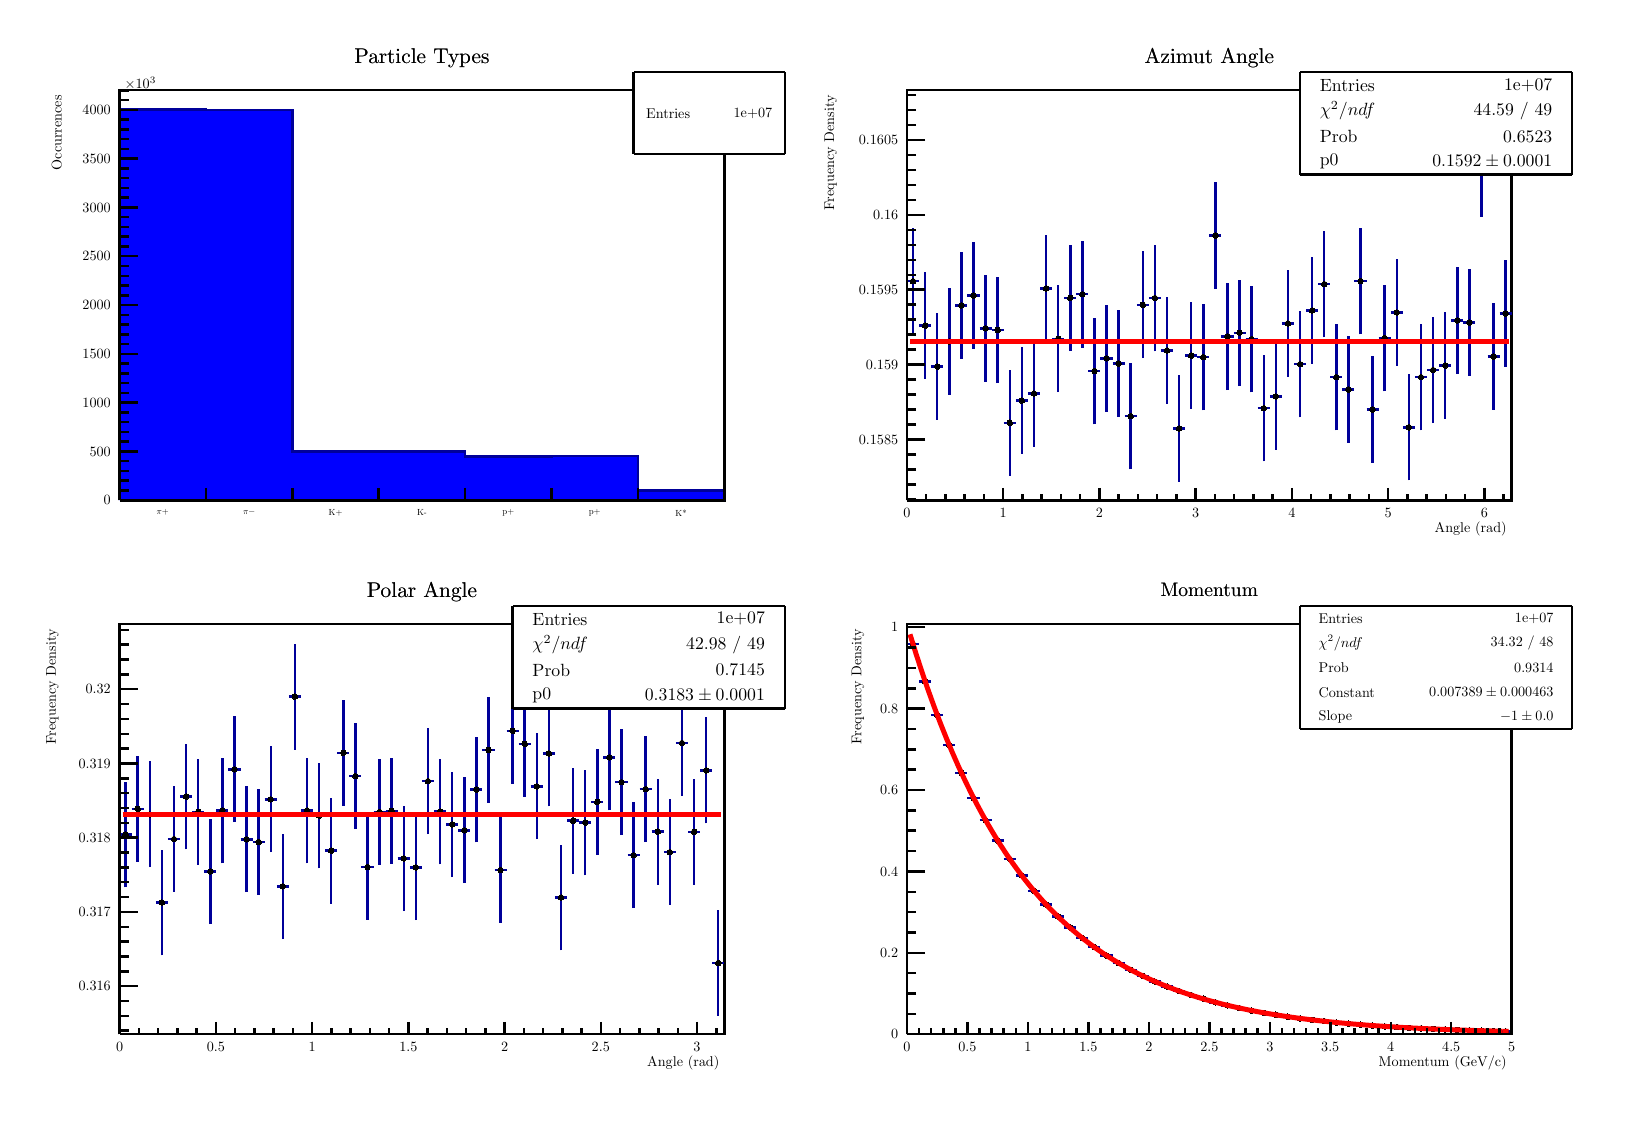
\begin{tikzpicture}
\pgfdeclareplotmark{cross} {
\pgfpathmoveto{\pgfpoint{-0.3\pgfplotmarksize}{\pgfplotmarksize}}
\pgfpathlineto{\pgfpoint{+0.3\pgfplotmarksize}{\pgfplotmarksize}}
\pgfpathlineto{\pgfpoint{+0.3\pgfplotmarksize}{0.3\pgfplotmarksize}}
\pgfpathlineto{\pgfpoint{+1\pgfplotmarksize}{0.3\pgfplotmarksize}}
\pgfpathlineto{\pgfpoint{+1\pgfplotmarksize}{-0.3\pgfplotmarksize}}
\pgfpathlineto{\pgfpoint{+0.3\pgfplotmarksize}{-0.3\pgfplotmarksize}}
\pgfpathlineto{\pgfpoint{+0.3\pgfplotmarksize}{-1.\pgfplotmarksize}}
\pgfpathlineto{\pgfpoint{-0.3\pgfplotmarksize}{-1.\pgfplotmarksize}}
\pgfpathlineto{\pgfpoint{-0.3\pgfplotmarksize}{-0.3\pgfplotmarksize}}
\pgfpathlineto{\pgfpoint{-1.\pgfplotmarksize}{-0.3\pgfplotmarksize}}
\pgfpathlineto{\pgfpoint{-1.\pgfplotmarksize}{0.3\pgfplotmarksize}}
\pgfpathlineto{\pgfpoint{-0.3\pgfplotmarksize}{0.3\pgfplotmarksize}}
\pgfpathclose
\pgfusepathqstroke
}
\pgfdeclareplotmark{cross*} {
\pgfpathmoveto{\pgfpoint{-0.3\pgfplotmarksize}{\pgfplotmarksize}}
\pgfpathlineto{\pgfpoint{+0.3\pgfplotmarksize}{\pgfplotmarksize}}
\pgfpathlineto{\pgfpoint{+0.3\pgfplotmarksize}{0.3\pgfplotmarksize}}
\pgfpathlineto{\pgfpoint{+1\pgfplotmarksize}{0.3\pgfplotmarksize}}
\pgfpathlineto{\pgfpoint{+1\pgfplotmarksize}{-0.3\pgfplotmarksize}}
\pgfpathlineto{\pgfpoint{+0.3\pgfplotmarksize}{-0.3\pgfplotmarksize}}
\pgfpathlineto{\pgfpoint{+0.3\pgfplotmarksize}{-1.\pgfplotmarksize}}
\pgfpathlineto{\pgfpoint{-0.3\pgfplotmarksize}{-1.\pgfplotmarksize}}
\pgfpathlineto{\pgfpoint{-0.3\pgfplotmarksize}{-0.3\pgfplotmarksize}}
\pgfpathlineto{\pgfpoint{-1.\pgfplotmarksize}{-0.3\pgfplotmarksize}}
\pgfpathlineto{\pgfpoint{-1.\pgfplotmarksize}{0.3\pgfplotmarksize}}
\pgfpathlineto{\pgfpoint{-0.3\pgfplotmarksize}{0.3\pgfplotmarksize}}
\pgfpathclose
\pgfusepathqfillstroke
}
\pgfdeclareplotmark{newstar} {
\pgfpathmoveto{\pgfqpoint{0pt}{\pgfplotmarksize}}
\pgfpathlineto{\pgfqpointpolar{44}{0.5\pgfplotmarksize}}
\pgfpathlineto{\pgfqpointpolar{18}{\pgfplotmarksize}}
\pgfpathlineto{\pgfqpointpolar{-20}{0.5\pgfplotmarksize}}
\pgfpathlineto{\pgfqpointpolar{-54}{\pgfplotmarksize}}
\pgfpathlineto{\pgfqpointpolar{-90}{0.5\pgfplotmarksize}}
\pgfpathlineto{\pgfqpointpolar{234}{\pgfplotmarksize}}
\pgfpathlineto{\pgfqpointpolar{198}{0.5\pgfplotmarksize}}
\pgfpathlineto{\pgfqpointpolar{162}{\pgfplotmarksize}}
\pgfpathlineto{\pgfqpointpolar{134}{0.5\pgfplotmarksize}}
\pgfpathclose
\pgfusepathqstroke
}
\pgfdeclareplotmark{newstar*} {
\pgfpathmoveto{\pgfqpoint{0pt}{\pgfplotmarksize}}
\pgfpathlineto{\pgfqpointpolar{44}{0.5\pgfplotmarksize}}
\pgfpathlineto{\pgfqpointpolar{18}{\pgfplotmarksize}}
\pgfpathlineto{\pgfqpointpolar{-20}{0.5\pgfplotmarksize}}
\pgfpathlineto{\pgfqpointpolar{-54}{\pgfplotmarksize}}
\pgfpathlineto{\pgfqpointpolar{-90}{0.5\pgfplotmarksize}}
\pgfpathlineto{\pgfqpointpolar{234}{\pgfplotmarksize}}
\pgfpathlineto{\pgfqpointpolar{198}{0.5\pgfplotmarksize}}
\pgfpathlineto{\pgfqpointpolar{162}{\pgfplotmarksize}}
\pgfpathlineto{\pgfqpointpolar{134}{0.5\pgfplotmarksize}}
\pgfpathclose
\pgfusepathqfillstroke
}
\definecolor{c}{rgb}{1,1,1};
\draw [color=c, fill=c] (0,0) rectangle (20,13.5632);
\draw [color=c, fill=c] (0.2,6.91724) rectangle (9.8,13.4276);
\draw [color=c, fill=c] (1.16,7.56828) rectangle (8.84,12.7766);
\definecolor{c}{rgb}{0,0,0};
\draw [c,line width=0.9] (1.16,7.56828) -- (1.16,12.7766) -- (8.84,12.7766) -- (8.84,7.56828) -- (1.16,7.56828);
\definecolor{c}{rgb}{0,0,1};
\draw [c, fill=c] (1.16,7.56828) -- (1.16,12.5285) -- (2.25714,12.5285) -- (2.25714,12.5254) -- (3.35429,12.5254) -- (3.35429,8.18713) -- (4.45143,8.18713) -- (4.45143,8.18721) -- (5.54857,8.18721) -- (5.54857,8.12575) -- (6.64571,8.12575) --
 (6.64571,8.12734) -- (7.74286,8.12734) -- (7.74286,7.69282) -- (8.84,7.69282) -- (8.84,7.56828);
\definecolor{c}{rgb}{0,0,0.6};
\draw [c,line width=0.9] (1.16,12.5285) -- (2.25714,12.5285) -- (2.25714,12.5254) -- (3.35429,12.5254) -- (3.35429,8.18713) -- (4.45143,8.18713) -- (4.45143,8.18721) -- (5.54857,8.18721) -- (5.54857,8.12575) -- (6.64571,8.12575) -- (6.64571,8.12734)
 -- (7.74286,8.12734) -- (7.74286,7.69282) -- (8.84,7.69282);
\definecolor{c}{rgb}{0,0,0};
\draw [c,line width=0.9] (1.16,7.56828) -- (8.84,7.56828);
\draw [anchor=north] (1.70857,7.49015) node[scale=0.319896, color=c, rotate=0]{$\pi+$};
\draw [anchor=north] (2.80571,7.49015) node[scale=0.319896, color=c, rotate=0]{$\pi-$};
\draw [anchor=north] (3.90286,7.49015) node[scale=0.319896, color=c, rotate=0]{K+};
\draw [anchor=north] (5,7.49015) node[scale=0.319896, color=c, rotate=0]{K-};
\draw [anchor=north] (6.09714,7.49015) node[scale=0.319896, color=c, rotate=0]{p+};
\draw [anchor=north] (7.19429,7.49015) node[scale=0.319896, color=c, rotate=0]{p+};
\draw [anchor=north] (8.29143,7.49015) node[scale=0.319896, color=c, rotate=0]{K*};
\draw [c,line width=0.9] (1.16,7.72452) -- (1.16,7.56828);
\draw [c,line width=0.9] (2.25714,7.72452) -- (2.25714,7.56828);
\draw [c,line width=0.9] (3.35429,7.72452) -- (3.35429,7.56828);
\draw [c,line width=0.9] (4.45143,7.72452) -- (4.45143,7.56828);
\draw [c,line width=0.9] (5.54857,7.72452) -- (5.54857,7.56828);
\draw [c,line width=0.9] (6.64571,7.72452) -- (6.64571,7.56828);
\draw [c,line width=0.9] (7.74286,7.72452) -- (7.74286,7.56828);
\draw [c,line width=0.9] (8.84,7.72452) -- (8.84,7.56828);
\draw [c,line width=0.9] (1.16,7.56828) -- (1.16,12.7766);
\draw [c,line width=0.9] (1.3904,7.56828) -- (1.16,7.56828);
\draw [c,line width=0.9] (1.2752,7.69224) -- (1.16,7.69224);
\draw [c,line width=0.9] (1.2752,7.8162) -- (1.16,7.8162);
\draw [c,line width=0.9] (1.2752,7.94016) -- (1.16,7.94016);
\draw [c,line width=0.9] (1.2752,8.06413) -- (1.16,8.06413);
\draw [c,line width=0.9] (1.3904,8.18809) -- (1.16,8.18809);
\draw [c,line width=0.9] (1.2752,8.31205) -- (1.16,8.31205);
\draw [c,line width=0.9] (1.2752,8.43601) -- (1.16,8.43601);
\draw [c,line width=0.9] (1.2752,8.55998) -- (1.16,8.55998);
\draw [c,line width=0.9] (1.2752,8.68394) -- (1.16,8.68394);
\draw [c,line width=0.9] (1.3904,8.8079) -- (1.16,8.8079);
\draw [c,line width=0.9] (1.2752,8.93186) -- (1.16,8.93186);
\draw [c,line width=0.9] (1.2752,9.05583) -- (1.16,9.05583);
\draw [c,line width=0.9] (1.2752,9.17979) -- (1.16,9.17979);
\draw [c,line width=0.9] (1.2752,9.30375) -- (1.16,9.30375);
\draw [c,line width=0.9] (1.3904,9.42771) -- (1.16,9.42771);
\draw [c,line width=0.9] (1.2752,9.55168) -- (1.16,9.55168);
\draw [c,line width=0.9] (1.2752,9.67564) -- (1.16,9.67564);
\draw [c,line width=0.9] (1.2752,9.7996) -- (1.16,9.7996);
\draw [c,line width=0.9] (1.2752,9.92356) -- (1.16,9.92356);
\draw [c,line width=0.9] (1.3904,10.0475) -- (1.16,10.0475);
\draw [c,line width=0.9] (1.2752,10.1715) -- (1.16,10.1715);
\draw [c,line width=0.9] (1.2752,10.2955) -- (1.16,10.2955);
\draw [c,line width=0.9] (1.2752,10.4194) -- (1.16,10.4194);
\draw [c,line width=0.9] (1.2752,10.5434) -- (1.16,10.5434);
\draw [c,line width=0.9] (1.3904,10.6673) -- (1.16,10.6673);
\draw [c,line width=0.9] (1.2752,10.7913) -- (1.16,10.7913);
\draw [c,line width=0.9] (1.2752,10.9153) -- (1.16,10.9153);
\draw [c,line width=0.9] (1.2752,11.0392) -- (1.16,11.0392);
\draw [c,line width=0.9] (1.2752,11.1632) -- (1.16,11.1632);
\draw [c,line width=0.9] (1.3904,11.2872) -- (1.16,11.2872);
\draw [c,line width=0.9] (1.2752,11.4111) -- (1.16,11.4111);
\draw [c,line width=0.9] (1.2752,11.5351) -- (1.16,11.5351);
\draw [c,line width=0.9] (1.2752,11.659) -- (1.16,11.659);
\draw [c,line width=0.9] (1.2752,11.783) -- (1.16,11.783);
\draw [c,line width=0.9] (1.3904,11.907) -- (1.16,11.907);
\draw [c,line width=0.9] (1.2752,12.0309) -- (1.16,12.0309);
\draw [c,line width=0.9] (1.2752,12.1549) -- (1.16,12.1549);
\draw [c,line width=0.9] (1.2752,12.2789) -- (1.16,12.2789);
\draw [c,line width=0.9] (1.2752,12.4028) -- (1.16,12.4028);
\draw [c,line width=0.9] (1.3904,12.5268) -- (1.16,12.5268);
\draw [c,line width=0.9] (1.3904,12.5268) -- (1.16,12.5268);
\draw [c,line width=0.9] (1.2752,12.6507) -- (1.16,12.6507);
\draw [c,line width=0.9] (1.2752,12.7747) -- (1.16,12.7747);
\draw [anchor= east] (1.112,7.56828) node[scale=0.511833, color=c, rotate=0]{0};
\draw [anchor= east] (1.112,8.18809) node[scale=0.511833, color=c, rotate=0]{500};
\draw [anchor= east] (1.112,8.8079) node[scale=0.511833, color=c, rotate=0]{1000};
\draw [anchor= east] (1.112,9.42771) node[scale=0.511833, color=c, rotate=0]{1500};
\draw [anchor= east] (1.112,10.0475) node[scale=0.511833, color=c, rotate=0]{2000};
\draw [anchor= east] (1.112,10.6673) node[scale=0.511833, color=c, rotate=0]{2500};
\draw [anchor= east] (1.112,11.2872) node[scale=0.511833, color=c, rotate=0]{3000};
\draw [anchor= east] (1.112,11.907) node[scale=0.511833, color=c, rotate=0]{3500};
\draw [anchor= east] (1.112,12.5268) node[scale=0.511833, color=c, rotate=0]{4000};
\draw [anchor=base west] (1.16,12.7993) node[scale=0.511833, color=c, rotate=0]{$\times10^{3}$};
\draw [anchor= east] (0.36423,12.7766) node[scale=0.511833, color=c, rotate=90]{Occurrences};
\draw (5,13.1881) node[scale=0.767749, color=c, rotate=0]{Particle Types};
\definecolor{c}{rgb}{1,1,1};
\draw [color=c, fill=c] (7.688,11.9628) rectangle (9.608,13.0044);
\definecolor{c}{rgb}{0,0,0};
\draw [c,line width=0.9] (7.688,11.9628) -- (9.608,11.9628);
\draw [c,line width=0.9] (9.608,11.9628) -- (9.608,13.0044);
\draw [c,line width=0.9] (9.608,13.0044) -- (7.688,13.0044);
\draw [c,line width=0.9] (7.688,13.0044) -- (7.688,11.9628);
\draw [anchor= west] (7.784,12.4836) node[scale=0.511833, color=c, rotate=0]{Entries };
\draw [anchor= east] (9.512,12.4836) node[scale=0.511833, color=c, rotate=0]{          1e+07};
\draw (5,13.1881) node[scale=0.767749, color=c, rotate=0]{Particle Types};
\definecolor{c}{rgb}{1,1,1};
\draw [color=c, fill=c] (10.2,6.91724) rectangle (19.8,13.4276);
\draw [color=c, fill=c] (11.16,7.56828) rectangle (18.84,12.7766);
\definecolor{c}{rgb}{0,0,0};
\draw [c,line width=0.9] (11.16,7.56828) -- (11.16,12.7766) -- (18.84,12.7766) -- (18.84,7.56828) -- (11.16,7.56828);
\definecolor{c}{rgb}{0,0,0.6};
\draw [c,line width=0.9] (11.2368,9.67248) -- (11.2368,10.35);
\draw [c,line width=0.9] (11.2368,10.35) -- (11.2368,11.0275);
\draw [c,line width=0.9] (11.16,10.35) -- (11.2368,10.35);
\draw [c,line width=0.9] (11.2368,10.35) -- (11.3136,10.35);
\definecolor{c}{rgb}{0,0,0};
\foreach \P in {(11.2368,10.35)}{\draw[mark options={color=c,fill=c},mark size=2.402402pt, line width=0.000000pt, mark=*,mark size=1pt] plot coordinates {\P};}
\definecolor{c}{rgb}{0,0,0.6};
\draw [c,line width=0.9] (11.3904,9.10875) -- (11.3904,9.78562);
\draw [c,line width=0.9] (11.3904,9.78562) -- (11.3904,10.4625);
\draw [c,line width=0.9] (11.3136,9.78562) -- (11.3904,9.78562);
\draw [c,line width=0.9] (11.3904,9.78562) -- (11.4672,9.78562);
\definecolor{c}{rgb}{0,0,0};
\foreach \P in {(11.3904,9.78562)}{\draw[mark options={color=c,fill=c},mark size=2.402402pt, line width=0.000000pt, mark=*,mark size=1pt] plot coordinates {\P};}
\definecolor{c}{rgb}{0,0,0.6};
\draw [c,line width=0.9] (11.544,8.58886) -- (11.544,9.26514);
\draw [c,line width=0.9] (11.544,9.26514) -- (11.544,9.94142);
\draw [c,line width=0.9] (11.4672,9.26514) -- (11.544,9.26514);
\draw [c,line width=0.9] (11.544,9.26514) -- (11.6208,9.26514);
\definecolor{c}{rgb}{0,0,0};
\foreach \P in {(11.544,9.26514)}{\draw[mark options={color=c,fill=c},mark size=2.402402pt, line width=0.000000pt, mark=*,mark size=1pt] plot coordinates {\P};}
\definecolor{c}{rgb}{0,0,0.6};
\draw [c,line width=0.9] (11.6976,8.90774) -- (11.6976,9.58438);
\draw [c,line width=0.9] (11.6976,9.58438) -- (11.6976,10.261);
\draw [c,line width=0.9] (11.6208,9.58438) -- (11.6976,9.58438);
\draw [c,line width=0.9] (11.6976,9.58438) -- (11.7744,9.58438);
\definecolor{c}{rgb}{0,0,0};
\foreach \P in {(11.6976,9.58438)}{\draw[mark options={color=c,fill=c},mark size=2.402402pt, line width=0.000000pt, mark=*,mark size=1pt] plot coordinates {\P};}
\definecolor{c}{rgb}{0,0,0.6};
\draw [c,line width=0.9] (11.8512,9.36568) -- (11.8512,10.0428);
\draw [c,line width=0.9] (11.8512,10.0428) -- (11.8512,10.72);
\draw [c,line width=0.9] (11.7744,10.0428) -- (11.8512,10.0428);
\draw [c,line width=0.9] (11.8512,10.0428) -- (11.928,10.0428);
\definecolor{c}{rgb}{0,0,0};
\foreach \P in {(11.8512,10.0428)}{\draw[mark options={color=c,fill=c},mark size=2.402402pt, line width=0.000000pt, mark=*,mark size=1pt] plot coordinates {\P};}
\definecolor{c}{rgb}{0,0,0.6};
\draw [c,line width=0.9] (12.0048,9.49112) -- (12.0048,10.1684);
\draw [c,line width=0.9] (12.0048,10.1684) -- (12.0048,10.8457);
\draw [c,line width=0.9] (11.928,10.1684) -- (12.0048,10.1684);
\draw [c,line width=0.9] (12.0048,10.1684) -- (12.0816,10.1684);
\definecolor{c}{rgb}{0,0,0};
\foreach \P in {(12.0048,10.1684)}{\draw[mark options={color=c,fill=c},mark size=2.402402pt, line width=0.000000pt, mark=*,mark size=1pt] plot coordinates {\P};}
\definecolor{c}{rgb}{0,0,0.6};
\draw [c,line width=0.9] (12.1584,9.0755) -- (12.1584,9.75233);
\draw [c,line width=0.9] (12.1584,9.75233) -- (12.1584,10.4292);
\draw [c,line width=0.9] (12.0816,9.75233) -- (12.1584,9.75233);
\draw [c,line width=0.9] (12.1584,9.75233) -- (12.2352,9.75233);
\definecolor{c}{rgb}{0,0,0};
\foreach \P in {(12.1584,9.75233)}{\draw[mark options={color=c,fill=c},mark size=2.402402pt, line width=0.000000pt, mark=*,mark size=1pt] plot coordinates {\P};}
\definecolor{c}{rgb}{0,0,0.6};
\draw [c,line width=0.9] (12.312,9.05434) -- (12.312,9.73115);
\draw [c,line width=0.9] (12.312,9.73115) -- (12.312,10.408);
\draw [c,line width=0.9] (12.2352,9.73115) -- (12.312,9.73115);
\draw [c,line width=0.9] (12.312,9.73115) -- (12.3888,9.73115);
\definecolor{c}{rgb}{0,0,0};
\foreach \P in {(12.312,9.73115)}{\draw[mark options={color=c,fill=c},mark size=2.402402pt, line width=0.000000pt, mark=*,mark size=1pt] plot coordinates {\P};}
\definecolor{c}{rgb}{0,0,0.6};
\draw [c,line width=0.9] (12.4656,7.87702) -- (12.4656,8.55251);
\draw [c,line width=0.9] (12.4656,8.55251) -- (12.4656,9.22799);
\draw [c,line width=0.9] (12.3888,8.55251) -- (12.4656,8.55251);
\draw [c,line width=0.9] (12.4656,8.55251) -- (12.5424,8.55251);
\definecolor{c}{rgb}{0,0,0};
\foreach \P in {(12.4656,8.55251)}{\draw[mark options={color=c,fill=c},mark size=2.402402pt, line width=0.000000pt, mark=*,mark size=1pt] plot coordinates {\P};}
\definecolor{c}{rgb}{0,0,0.6};
\draw [c,line width=0.9] (12.6192,8.15813) -- (12.6192,8.83393);
\draw [c,line width=0.9] (12.6192,8.83393) -- (12.6192,9.50973);
\draw [c,line width=0.9] (12.5424,8.83393) -- (12.6192,8.83393);
\draw [c,line width=0.9] (12.6192,8.83393) -- (12.696,8.83393);
\definecolor{c}{rgb}{0,0,0};
\foreach \P in {(12.6192,8.83393)}{\draw[mark options={color=c,fill=c},mark size=2.402402pt, line width=0.000000pt, mark=*,mark size=1pt] plot coordinates {\P};}
\definecolor{c}{rgb}{0,0,0.6};
\draw [c,line width=0.9] (12.7728,8.24881) -- (12.7728,8.92471);
\draw [c,line width=0.9] (12.7728,8.92471) -- (12.7728,9.60061);
\draw [c,line width=0.9] (12.696,8.92471) -- (12.7728,8.92471);
\draw [c,line width=0.9] (12.7728,8.92471) -- (12.8496,8.92471);
\definecolor{c}{rgb}{0,0,0};
\foreach \P in {(12.7728,8.92471)}{\draw[mark options={color=c,fill=c},mark size=2.402402pt, line width=0.000000pt, mark=*,mark size=1pt] plot coordinates {\P};}
\definecolor{c}{rgb}{0,0,0.6};
\draw [c,line width=0.9] (12.9264,9.5818) -- (12.9264,10.2592);
\draw [c,line width=0.9] (12.9264,10.2592) -- (12.9264,10.9366);
\draw [c,line width=0.9] (12.8496,10.2592) -- (12.9264,10.2592);
\draw [c,line width=0.9] (12.9264,10.2592) -- (13.0032,10.2592);
\definecolor{c}{rgb}{0,0,0};
\foreach \P in {(12.9264,10.2592)}{\draw[mark options={color=c,fill=c},mark size=2.402402pt, line width=0.000000pt, mark=*,mark size=1pt] plot coordinates {\P};}
\definecolor{c}{rgb}{0,0,0.6};
\draw [c,line width=0.9] (13.08,8.94251) -- (13.08,9.61918);
\draw [c,line width=0.9] (13.08,9.61918) -- (13.08,10.2959);
\draw [c,line width=0.9] (13.0032,9.61918) -- (13.08,9.61918);
\draw [c,line width=0.9] (13.08,9.61918) -- (13.1568,9.61918);
\definecolor{c}{rgb}{0,0,0};
\foreach \P in {(13.08,9.61918)}{\draw[mark options={color=c,fill=c},mark size=2.402402pt, line width=0.000000pt, mark=*,mark size=1pt] plot coordinates {\P};}
\definecolor{c}{rgb}{0,0,0.6};
\draw [c,line width=0.9] (13.2336,9.46089) -- (13.2336,10.1381);
\draw [c,line width=0.9] (13.2336,10.1381) -- (13.2336,10.8154);
\draw [c,line width=0.9] (13.1568,10.1381) -- (13.2336,10.1381);
\draw [c,line width=0.9] (13.2336,10.1381) -- (13.3104,10.1381);
\definecolor{c}{rgb}{0,0,0};
\foreach \P in {(13.2336,10.1381)}{\draw[mark options={color=c,fill=c},mark size=2.402402pt, line width=0.000000pt, mark=*,mark size=1pt] plot coordinates {\P};}
\definecolor{c}{rgb}{0,0,0.6};
\draw [c,line width=0.9] (13.3872,9.50774) -- (13.3872,10.1851);
\draw [c,line width=0.9] (13.3872,10.1851) -- (13.3872,10.8624);
\draw [c,line width=0.9] (13.3104,10.1851) -- (13.3872,10.1851);
\draw [c,line width=0.9] (13.3872,10.1851) -- (13.464,10.1851);
\definecolor{c}{rgb}{0,0,0};
\foreach \P in {(13.3872,10.1851)}{\draw[mark options={color=c,fill=c},mark size=2.402402pt, line width=0.000000pt, mark=*,mark size=1pt] plot coordinates {\P};}
\definecolor{c}{rgb}{0,0,0.6};
\draw [c,line width=0.9] (13.5408,8.53294) -- (13.5408,9.20916);
\draw [c,line width=0.9] (13.5408,9.20916) -- (13.5408,9.88538);
\draw [c,line width=0.9] (13.464,9.20916) -- (13.5408,9.20916);
\draw [c,line width=0.9] (13.5408,9.20916) -- (13.6176,9.20916);
\definecolor{c}{rgb}{0,0,0};
\foreach \P in {(13.5408,9.20916)}{\draw[mark options={color=c,fill=c},mark size=2.402402pt, line width=0.000000pt, mark=*,mark size=1pt] plot coordinates {\P};}
\definecolor{c}{rgb}{0,0,0.6};
\draw [c,line width=0.9] (13.6944,8.69465) -- (13.6944,9.37105);
\draw [c,line width=0.9] (13.6944,9.37105) -- (13.6944,10.0475);
\draw [c,line width=0.9] (13.6176,9.37105) -- (13.6944,9.37105);
\draw [c,line width=0.9] (13.6944,9.37105) -- (13.7712,9.37105);
\definecolor{c}{rgb}{0,0,0};
\foreach \P in {(13.6944,9.37105)}{\draw[mark options={color=c,fill=c},mark size=2.402402pt, line width=0.000000pt, mark=*,mark size=1pt] plot coordinates {\P};}
\definecolor{c}{rgb}{0,0,0.6};
\draw [c,line width=0.9] (13.848,8.62815) -- (13.848,9.30448);
\draw [c,line width=0.9] (13.848,9.30448) -- (13.848,9.9808);
\draw [c,line width=0.9] (13.7712,9.30448) -- (13.848,9.30448);
\draw [c,line width=0.9] (13.848,9.30448) -- (13.9248,9.30448);
\definecolor{c}{rgb}{0,0,0};
\foreach \P in {(13.848,9.30448)}{\draw[mark options={color=c,fill=c},mark size=2.402402pt, line width=0.000000pt, mark=*,mark size=1pt] plot coordinates {\P};}
\definecolor{c}{rgb}{0,0,0.6};
\draw [c,line width=0.9] (14.0016,7.96014) -- (14.0016,8.63572);
\draw [c,line width=0.9] (14.0016,8.63572) -- (14.0016,9.3113);
\draw [c,line width=0.9] (13.9248,8.63572) -- (14.0016,8.63572);
\draw [c,line width=0.9] (14.0016,8.63572) -- (14.0784,8.63572);
\definecolor{c}{rgb}{0,0,0};
\foreach \P in {(14.0016,8.63572)}{\draw[mark options={color=c,fill=c},mark size=2.402402pt, line width=0.000000pt, mark=*,mark size=1pt] plot coordinates {\P};}
\definecolor{c}{rgb}{0,0,0.6};
\draw [c,line width=0.9] (14.1552,9.37323) -- (14.1552,10.0504);
\draw [c,line width=0.9] (14.1552,10.0504) -- (14.1552,10.7276);
\draw [c,line width=0.9] (14.0784,10.0504) -- (14.1552,10.0504);
\draw [c,line width=0.9] (14.1552,10.0504) -- (14.232,10.0504);
\definecolor{c}{rgb}{0,0,0};
\foreach \P in {(14.1552,10.0504)}{\draw[mark options={color=c,fill=c},mark size=2.402402pt, line width=0.000000pt, mark=*,mark size=1pt] plot coordinates {\P};}
\definecolor{c}{rgb}{0,0,0.6};
\draw [c,line width=0.9] (14.3088,9.45938) -- (14.3088,10.1366);
\draw [c,line width=0.9] (14.3088,10.1366) -- (14.3088,10.8139);
\draw [c,line width=0.9] (14.232,10.1366) -- (14.3088,10.1366);
\draw [c,line width=0.9] (14.3088,10.1366) -- (14.3856,10.1366);
\definecolor{c}{rgb}{0,0,0};
\foreach \P in {(14.3088,10.1366)}{\draw[mark options={color=c,fill=c},mark size=2.402402pt, line width=0.000000pt, mark=*,mark size=1pt] plot coordinates {\P};}
\definecolor{c}{rgb}{0,0,0.6};
\draw [c,line width=0.9] (14.4624,8.7944) -- (14.4624,9.47091);
\draw [c,line width=0.9] (14.4624,9.47091) -- (14.4624,10.1474);
\draw [c,line width=0.9] (14.3856,9.47091) -- (14.4624,9.47091);
\draw [c,line width=0.9] (14.4624,9.47091) -- (14.5392,9.47091);
\definecolor{c}{rgb}{0,0,0};
\foreach \P in {(14.4624,9.47091)}{\draw[mark options={color=c,fill=c},mark size=2.402402pt, line width=0.000000pt, mark=*,mark size=1pt] plot coordinates {\P};}
\definecolor{c}{rgb}{0,0,0.6};
\draw [c,line width=0.9] (14.616,7.80448) -- (14.616,8.47988);
\draw [c,line width=0.9] (14.616,8.47988) -- (14.616,9.15529);
\draw [c,line width=0.9] (14.5392,8.47988) -- (14.616,8.47988);
\draw [c,line width=0.9] (14.616,8.47988) -- (14.6928,8.47988);
\definecolor{c}{rgb}{0,0,0};
\foreach \P in {(14.616,8.47988)}{\draw[mark options={color=c,fill=c},mark size=2.402402pt, line width=0.000000pt, mark=*,mark size=1pt] plot coordinates {\P};}
\definecolor{c}{rgb}{0,0,0.6};
\draw [c,line width=0.9] (14.7696,8.7279) -- (14.7696,9.40434);
\draw [c,line width=0.9] (14.7696,9.40434) -- (14.7696,10.0808);
\draw [c,line width=0.9] (14.6928,9.40434) -- (14.7696,9.40434);
\draw [c,line width=0.9] (14.7696,9.40434) -- (14.8464,9.40434);
\definecolor{c}{rgb}{0,0,0};
\foreach \P in {(14.7696,9.40434)}{\draw[mark options={color=c,fill=c},mark size=2.402402pt, line width=0.000000pt, mark=*,mark size=1pt] plot coordinates {\P};}
\definecolor{c}{rgb}{0,0,0.6};
\draw [c,line width=0.9] (14.9232,8.70976) -- (14.9232,9.38618);
\draw [c,line width=0.9] (14.9232,9.38618) -- (14.9232,10.0626);
\draw [c,line width=0.9] (14.8464,9.38618) -- (14.9232,9.38618);
\draw [c,line width=0.9] (14.9232,9.38618) -- (15,9.38618);
\definecolor{c}{rgb}{0,0,0};
\foreach \P in {(14.9232,9.38618)}{\draw[mark options={color=c,fill=c},mark size=2.402402pt, line width=0.000000pt, mark=*,mark size=1pt] plot coordinates {\P};}
\definecolor{c}{rgb}{0,0,0.6};
\draw [c,line width=0.9] (15.0768,10.2498) -- (15.0768,10.9279);
\draw [c,line width=0.9] (15.0768,10.9279) -- (15.0768,11.6061);
\draw [c,line width=0.9] (15,10.9279) -- (15.0768,10.9279);
\draw [c,line width=0.9] (15.0768,10.9279) -- (15.1536,10.9279);
\definecolor{c}{rgb}{0,0,0};
\foreach \P in {(15.0768,10.9279)}{\draw[mark options={color=c,fill=c},mark size=2.402402pt, line width=0.000000pt, mark=*,mark size=1pt] plot coordinates {\P};}
\definecolor{c}{rgb}{0,0,0.6};
\draw [c,line width=0.9] (15.2304,8.9682) -- (15.2304,9.64491);
\draw [c,line width=0.9] (15.2304,9.64491) -- (15.2304,10.3216);
\draw [c,line width=0.9] (15.1536,9.64491) -- (15.2304,9.64491);
\draw [c,line width=0.9] (15.2304,9.64491) -- (15.3072,9.64491);
\definecolor{c}{rgb}{0,0,0};
\foreach \P in {(15.2304,9.64491)}{\draw[mark options={color=c,fill=c},mark size=2.402402pt, line width=0.000000pt, mark=*,mark size=1pt] plot coordinates {\P};}
\definecolor{c}{rgb}{0,0,0.6};
\draw [c,line width=0.9] (15.384,9.01807) -- (15.384,9.69483);
\draw [c,line width=0.9] (15.384,9.69483) -- (15.384,10.3716);
\draw [c,line width=0.9] (15.3072,9.69483) -- (15.384,9.69483);
\draw [c,line width=0.9] (15.384,9.69483) -- (15.4608,9.69483);
\definecolor{c}{rgb}{0,0,0};
\foreach \P in {(15.384,9.69483)}{\draw[mark options={color=c,fill=c},mark size=2.402402pt, line width=0.000000pt, mark=*,mark size=1pt] plot coordinates {\P};}
\definecolor{c}{rgb}{0,0,0.6};
\draw [c,line width=0.9] (15.5376,8.93797) -- (15.5376,9.61465);
\draw [c,line width=0.9] (15.5376,9.61465) -- (15.5376,10.2913);
\draw [c,line width=0.9] (15.4608,9.61465) -- (15.5376,9.61465);
\draw [c,line width=0.9] (15.5376,9.61465) -- (15.6144,9.61465);
\definecolor{c}{rgb}{0,0,0};
\foreach \P in {(15.5376,9.61465)}{\draw[mark options={color=c,fill=c},mark size=2.402402pt, line width=0.000000pt, mark=*,mark size=1pt] plot coordinates {\P};}
\definecolor{c}{rgb}{0,0,0.6};
\draw [c,line width=0.9] (15.6912,8.0614) -- (15.6912,8.7371);
\draw [c,line width=0.9] (15.6912,8.7371) -- (15.6912,9.41279);
\draw [c,line width=0.9] (15.6144,8.7371) -- (15.6912,8.7371);
\draw [c,line width=0.9] (15.6912,8.7371) -- (15.768,8.7371);
\definecolor{c}{rgb}{0,0,0};
\foreach \P in {(15.6912,8.7371)}{\draw[mark options={color=c,fill=c},mark size=2.402402pt, line width=0.000000pt, mark=*,mark size=1pt] plot coordinates {\P};}
\definecolor{c}{rgb}{0,0,0.6};
\draw [c,line width=0.9] (15.8448,8.21102) -- (15.8448,8.88688);
\draw [c,line width=0.9] (15.8448,8.88688) -- (15.8448,9.56274);
\draw [c,line width=0.9] (15.768,8.88688) -- (15.8448,8.88688);
\draw [c,line width=0.9] (15.8448,8.88688) -- (15.9216,8.88688);
\definecolor{c}{rgb}{0,0,0};
\foreach \P in {(15.8448,8.88688)}{\draw[mark options={color=c,fill=c},mark size=2.402402pt, line width=0.000000pt, mark=*,mark size=1pt] plot coordinates {\P};}
\definecolor{c}{rgb}{0,0,0.6};
\draw [c,line width=0.9] (15.9984,9.13747) -- (15.9984,9.81436);
\draw [c,line width=0.9] (15.9984,9.81436) -- (15.9984,10.4913);
\draw [c,line width=0.9] (15.9216,9.81436) -- (15.9984,9.81436);
\draw [c,line width=0.9] (15.9984,9.81436) -- (16.0752,9.81436);
\definecolor{c}{rgb}{0,0,0};
\foreach \P in {(15.9984,9.81436)}{\draw[mark options={color=c,fill=c},mark size=2.402402pt, line width=0.000000pt, mark=*,mark size=1pt] plot coordinates {\P};}
\definecolor{c}{rgb}{0,0,0.6};
\draw [c,line width=0.9] (16.152,8.62059) -- (16.152,9.29691);
\draw [c,line width=0.9] (16.152,9.29691) -- (16.152,9.97323);
\draw [c,line width=0.9] (16.0752,9.29691) -- (16.152,9.29691);
\draw [c,line width=0.9] (16.152,9.29691) -- (16.2288,9.29691);
\definecolor{c}{rgb}{0,0,0};
\foreach \P in {(16.152,9.29691)}{\draw[mark options={color=c,fill=c},mark size=2.402402pt, line width=0.000000pt, mark=*,mark size=1pt] plot coordinates {\P};}
\definecolor{c}{rgb}{0,0,0.6};
\draw [c,line width=0.9] (16.3056,9.30069) -- (16.3056,9.97777);
\draw [c,line width=0.9] (16.3056,9.97777) -- (16.3056,10.6548);
\draw [c,line width=0.9] (16.2288,9.97777) -- (16.3056,9.97777);
\draw [c,line width=0.9] (16.3056,9.97777) -- (16.3824,9.97777);
\definecolor{c}{rgb}{0,0,0};
\foreach \P in {(16.3056,9.97777)}{\draw[mark options={color=c,fill=c},mark size=2.402402pt, line width=0.000000pt, mark=*,mark size=1pt] plot coordinates {\P};}
\definecolor{c}{rgb}{0,0,0.6};
\draw [c,line width=0.9] (16.4592,9.6362) -- (16.4592,10.3137);
\draw [c,line width=0.9] (16.4592,10.3137) -- (16.4592,10.9911);
\draw [c,line width=0.9] (16.3824,10.3137) -- (16.4592,10.3137);
\draw [c,line width=0.9] (16.4592,10.3137) -- (16.536,10.3137);
\definecolor{c}{rgb}{0,0,0};
\foreach \P in {(16.4592,10.3137)}{\draw[mark options={color=c,fill=c},mark size=2.402402pt, line width=0.000000pt, mark=*,mark size=1pt] plot coordinates {\P};}
\definecolor{c}{rgb}{0,0,0.6};
\draw [c,line width=0.9] (16.6128,8.45586) -- (16.6128,9.13199);
\draw [c,line width=0.9] (16.6128,9.13199) -- (16.6128,9.80813);
\draw [c,line width=0.9] (16.536,9.13199) -- (16.6128,9.13199);
\draw [c,line width=0.9] (16.6128,9.13199) -- (16.6896,9.13199);
\definecolor{c}{rgb}{0,0,0};
\foreach \P in {(16.6128,9.13199)}{\draw[mark options={color=c,fill=c},mark size=2.402402pt, line width=0.000000pt, mark=*,mark size=1pt] plot coordinates {\P};}
\definecolor{c}{rgb}{0,0,0.6};
\draw [c,line width=0.9] (16.7664,8.29868) -- (16.7664,8.97464);
\draw [c,line width=0.9] (16.7664,8.97464) -- (16.7664,9.6506);
\draw [c,line width=0.9] (16.6896,8.97464) -- (16.7664,8.97464);
\draw [c,line width=0.9] (16.7664,8.97464) -- (16.8432,8.97464);
\definecolor{c}{rgb}{0,0,0};
\foreach \P in {(16.7664,8.97464)}{\draw[mark options={color=c,fill=c},mark size=2.402402pt, line width=0.000000pt, mark=*,mark size=1pt] plot coordinates {\P};}
\definecolor{c}{rgb}{0,0,0.6};
\draw [c,line width=0.9] (16.92,9.67399) -- (16.92,10.3515);
\draw [c,line width=0.9] (16.92,10.3515) -- (16.92,11.029);
\draw [c,line width=0.9] (16.8432,10.3515) -- (16.92,10.3515);
\draw [c,line width=0.9] (16.92,10.3515) -- (16.9968,10.3515);
\definecolor{c}{rgb}{0,0,0};
\foreach \P in {(16.92,10.3515)}{\draw[mark options={color=c,fill=c},mark size=2.402402pt, line width=0.000000pt, mark=*,mark size=1pt] plot coordinates {\P};}
\definecolor{c}{rgb}{0,0,0.6};
\draw [c,line width=0.9] (17.0736,8.04327) -- (17.0736,8.71894);
\draw [c,line width=0.9] (17.0736,8.71894) -- (17.0736,9.39461);
\draw [c,line width=0.9] (16.9968,8.71894) -- (17.0736,8.71894);
\draw [c,line width=0.9] (17.0736,8.71894) -- (17.1504,8.71894);
\definecolor{c}{rgb}{0,0,0};
\foreach \P in {(17.0736,8.71894)}{\draw[mark options={color=c,fill=c},mark size=2.402402pt, line width=0.000000pt, mark=*,mark size=1pt] plot coordinates {\P};}
\definecolor{c}{rgb}{0,0,0.6};
\draw [c,line width=0.9] (17.2272,8.95157) -- (17.2272,9.62826);
\draw [c,line width=0.9] (17.2272,9.62826) -- (17.2272,10.305);
\draw [c,line width=0.9] (17.1504,9.62826) -- (17.2272,9.62826);
\draw [c,line width=0.9] (17.2272,9.62826) -- (17.304,9.62826);
\definecolor{c}{rgb}{0,0,0};
\foreach \P in {(17.2272,9.62826)}{\draw[mark options={color=c,fill=c},mark size=2.402402pt, line width=0.000000pt, mark=*,mark size=1pt] plot coordinates {\P};}
\definecolor{c}{rgb}{0,0,0.6};
\draw [c,line width=0.9] (17.3808,9.275) -- (17.3808,9.95205);
\draw [c,line width=0.9] (17.3808,9.95205) -- (17.3808,10.6291);
\draw [c,line width=0.9] (17.304,9.95205) -- (17.3808,9.95205);
\draw [c,line width=0.9] (17.3808,9.95205) -- (17.4576,9.95205);
\definecolor{c}{rgb}{0,0,0};
\foreach \P in {(17.3808,9.95205)}{\draw[mark options={color=c,fill=c},mark size=2.402402pt, line width=0.000000pt, mark=*,mark size=1pt] plot coordinates {\P};}
\definecolor{c}{rgb}{0,0,0.6};
\draw [c,line width=0.9] (17.5344,7.81959) -- (17.5344,8.49501);
\draw [c,line width=0.9] (17.5344,8.49501) -- (17.5344,9.17043);
\draw [c,line width=0.9] (17.4576,8.49501) -- (17.5344,8.49501);
\draw [c,line width=0.9] (17.5344,8.49501) -- (17.6112,8.49501);
\definecolor{c}{rgb}{0,0,0};
\foreach \P in {(17.5344,8.49501)}{\draw[mark options={color=c,fill=c},mark size=2.402402pt, line width=0.000000pt, mark=*,mark size=1pt] plot coordinates {\P};}
\definecolor{c}{rgb}{0,0,0.6};
\draw [c,line width=0.9] (17.688,8.45586) -- (17.688,9.13199);
\draw [c,line width=0.9] (17.688,9.13199) -- (17.688,9.80813);
\draw [c,line width=0.9] (17.6112,9.13199) -- (17.688,9.13199);
\draw [c,line width=0.9] (17.688,9.13199) -- (17.7648,9.13199);
\definecolor{c}{rgb}{0,0,0};
\foreach \P in {(17.688,9.13199)}{\draw[mark options={color=c,fill=c},mark size=2.402402pt, line width=0.000000pt, mark=*,mark size=1pt] plot coordinates {\P};}
\definecolor{c}{rgb}{0,0,0.6};
\draw [c,line width=0.9] (17.8416,8.54654) -- (17.8416,9.22277);
\draw [c,line width=0.9] (17.8416,9.22277) -- (17.8416,9.89901);
\draw [c,line width=0.9] (17.7648,9.22277) -- (17.8416,9.22277);
\draw [c,line width=0.9] (17.8416,9.22277) -- (17.9184,9.22277);
\definecolor{c}{rgb}{0,0,0};
\foreach \P in {(17.8416,9.22277)}{\draw[mark options={color=c,fill=c},mark size=2.402402pt, line width=0.000000pt, mark=*,mark size=1pt] plot coordinates {\P};}
\definecolor{c}{rgb}{0,0,0.6};
\draw [c,line width=0.9] (17.9952,8.60246) -- (17.9952,9.27876);
\draw [c,line width=0.9] (17.9952,9.27876) -- (17.9952,9.95505);
\draw [c,line width=0.9] (17.9184,9.27876) -- (17.9952,9.27876);
\draw [c,line width=0.9] (17.9952,9.27876) -- (18.072,9.27876);
\definecolor{c}{rgb}{0,0,0};
\foreach \P in {(17.9952,9.27876)}{\draw[mark options={color=c,fill=c},mark size=2.402402pt, line width=0.000000pt, mark=*,mark size=1pt] plot coordinates {\P};}
\definecolor{c}{rgb}{0,0,0.6};
\draw [c,line width=0.9] (18.1488,9.17525) -- (18.1488,9.85219);
\draw [c,line width=0.9] (18.1488,9.85219) -- (18.1488,10.5291);
\draw [c,line width=0.9] (18.072,9.85219) -- (18.1488,9.85219);
\draw [c,line width=0.9] (18.1488,9.85219) -- (18.2256,9.85219);
\definecolor{c}{rgb}{0,0,0};
\foreach \P in {(18.1488,9.85219)}{\draw[mark options={color=c,fill=c},mark size=2.402402pt, line width=0.000000pt, mark=*,mark size=1pt] plot coordinates {\P};}
\definecolor{c}{rgb}{0,0,0.6};
\draw [c,line width=0.9] (18.3024,9.14805) -- (18.3024,9.82495);
\draw [c,line width=0.9] (18.3024,9.82495) -- (18.3024,10.5019);
\draw [c,line width=0.9] (18.2256,9.82495) -- (18.3024,9.82495);
\draw [c,line width=0.9] (18.3024,9.82495) -- (18.3792,9.82495);
\definecolor{c}{rgb}{0,0,0};
\foreach \P in {(18.3024,9.82495)}{\draw[mark options={color=c,fill=c},mark size=2.402402pt, line width=0.000000pt, mark=*,mark size=1pt] plot coordinates {\P};}
\definecolor{c}{rgb}{0,0,0.6};
\draw [c,line width=0.9] (18.456,11.1702) -- (18.456,11.8494);
\draw [c,line width=0.9] (18.456,11.8494) -- (18.456,12.5285);
\draw [c,line width=0.9] (18.3792,11.8494) -- (18.456,11.8494);
\draw [c,line width=0.9] (18.456,11.8494) -- (18.5328,11.8494);
\definecolor{c}{rgb}{0,0,0};
\foreach \P in {(18.456,11.8494)}{\draw[mark options={color=c,fill=c},mark size=2.402402pt, line width=0.000000pt, mark=*,mark size=1pt] plot coordinates {\P};}
\definecolor{c}{rgb}{0,0,0.6};
\draw [c,line width=0.9] (18.6096,8.71581) -- (18.6096,9.39223);
\draw [c,line width=0.9] (18.6096,9.39223) -- (18.6096,10.0687);
\draw [c,line width=0.9] (18.5328,9.39223) -- (18.6096,9.39223);
\draw [c,line width=0.9] (18.6096,9.39223) -- (18.6864,9.39223);
\definecolor{c}{rgb}{0,0,0};
\foreach \P in {(18.6096,9.39223)}{\draw[mark options={color=c,fill=c},mark size=2.402402pt, line width=0.000000pt, mark=*,mark size=1pt] plot coordinates {\P};}
\definecolor{c}{rgb}{0,0,0.6};
\draw [c,line width=0.9] (18.7632,9.26291) -- (18.7632,9.93994);
\draw [c,line width=0.9] (18.7632,9.93994) -- (18.7632,10.617);
\draw [c,line width=0.9] (18.6864,9.93994) -- (18.7632,9.93994);
\draw [c,line width=0.9] (18.7632,9.93994) -- (18.84,9.93994);
\definecolor{c}{rgb}{0,0,0};
\foreach \P in {(18.7632,9.93994)}{\draw[mark options={color=c,fill=c},mark size=2.402402pt, line width=0.000000pt, mark=*,mark size=1pt] plot coordinates {\P};}
\definecolor{c}{rgb}{1,0,0};
\draw [c,line width=1.8] (11.1984,9.58455) -- (11.2752,9.58455) -- (11.352,9.58455) -- (11.4288,9.58455) -- (11.5056,9.58455) -- (11.5824,9.58455) -- (11.6592,9.58455) -- (11.736,9.58455) -- (11.8128,9.58455) -- (11.8896,9.58455) -- (11.9664,9.58455)
 -- (12.0432,9.58455) -- (12.12,9.58455) -- (12.1968,9.58455) -- (12.2736,9.58455) -- (12.3504,9.58455) -- (12.4272,9.58455) -- (12.504,9.58455) -- (12.5808,9.58455) -- (12.6576,9.58455) -- (12.7344,9.58455) -- (12.8112,9.58455) -- (12.888,9.58455)
 -- (12.9648,9.58455) -- (13.0416,9.58455) -- (13.1184,9.58455) -- (13.1952,9.58455) -- (13.272,9.58455) -- (13.3488,9.58455) -- (13.4256,9.58455) -- (13.5024,9.58455) -- (13.5792,9.58455) -- (13.656,9.58455) -- (13.7328,9.58455) -- (13.8096,9.58455)
 -- (13.8864,9.58455) -- (13.9632,9.58455) -- (14.04,9.58455) -- (14.1168,9.58455) -- (14.1936,9.58455) -- (14.2704,9.58455) -- (14.3472,9.58455) -- (14.424,9.58455) -- (14.5008,9.58455) -- (14.5776,9.58455) -- (14.6544,9.58455) -- (14.7312,9.58455)
 -- (14.808,9.58455) -- (14.8848,9.58455) -- (14.9616,9.58455);
\draw [c,line width=1.8] (14.9616,9.58455) -- (15.0384,9.58455) -- (15.1152,9.58455) -- (15.192,9.58455) -- (15.2688,9.58455) -- (15.3456,9.58455) -- (15.4224,9.58455) -- (15.4992,9.58455) -- (15.576,9.58455) -- (15.6528,9.58455) -- (15.7296,9.58455)
 -- (15.8064,9.58455) -- (15.8832,9.58455) -- (15.96,9.58455) -- (16.0368,9.58455) -- (16.1136,9.58455) -- (16.1904,9.58455) -- (16.2672,9.58455) -- (16.344,9.58455) -- (16.4208,9.58455) -- (16.4976,9.58455) -- (16.5744,9.58455) -- (16.6512,9.58455)
 -- (16.728,9.58455) -- (16.8048,9.58455) -- (16.8816,9.58455) -- (16.9584,9.58455) -- (17.0352,9.58455) -- (17.112,9.58455) -- (17.1888,9.58455) -- (17.2656,9.58455) -- (17.3424,9.58455) -- (17.4192,9.58455) -- (17.496,9.58455) -- (17.5728,9.58455)
 -- (17.6496,9.58455) -- (17.7264,9.58455) -- (17.8032,9.58455) -- (17.88,9.58455) -- (17.9568,9.58455) -- (18.0336,9.58455) -- (18.1104,9.58455) -- (18.1872,9.58455) -- (18.264,9.58455) -- (18.3408,9.58455) -- (18.4176,9.58455) -- (18.4944,9.58455)
 -- (18.5712,9.58455) -- (18.648,9.58455) -- (18.7248,9.58455);
\draw [c,line width=1.8] (18.7248,9.58455) -- (18.8016,9.58455);
\definecolor{c}{rgb}{0,0,0};
\draw [c,line width=0.9] (11.16,7.56828) -- (18.84,7.56828);
\draw [c,line width=0.9] (11.16,7.72452) -- (11.16,7.56828);
\draw [c,line width=0.9] (11.4045,7.6464) -- (11.4045,7.56828);
\draw [c,line width=0.9] (11.6489,7.6464) -- (11.6489,7.56828);
\draw [c,line width=0.9] (11.8934,7.6464) -- (11.8934,7.56828);
\draw [c,line width=0.9] (12.1378,7.6464) -- (12.1378,7.56828);
\draw [c,line width=0.9] (12.3823,7.72452) -- (12.3823,7.56828);
\draw [c,line width=0.9] (12.6268,7.6464) -- (12.6268,7.56828);
\draw [c,line width=0.9] (12.8712,7.6464) -- (12.8712,7.56828);
\draw [c,line width=0.9] (13.1157,7.6464) -- (13.1157,7.56828);
\draw [c,line width=0.9] (13.3602,7.6464) -- (13.3602,7.56828);
\draw [c,line width=0.9] (13.6046,7.72452) -- (13.6046,7.56828);
\draw [c,line width=0.9] (13.8491,7.6464) -- (13.8491,7.56828);
\draw [c,line width=0.9] (14.0935,7.6464) -- (14.0935,7.56828);
\draw [c,line width=0.9] (14.338,7.6464) -- (14.338,7.56828);
\draw [c,line width=0.9] (14.5825,7.6464) -- (14.5825,7.56828);
\draw [c,line width=0.9] (14.8269,7.72452) -- (14.8269,7.56828);
\draw [c,line width=0.9] (15.0714,7.6464) -- (15.0714,7.56828);
\draw [c,line width=0.9] (15.3159,7.6464) -- (15.3159,7.56828);
\draw [c,line width=0.9] (15.5603,7.6464) -- (15.5603,7.56828);
\draw [c,line width=0.9] (15.8048,7.6464) -- (15.8048,7.56828);
\draw [c,line width=0.9] (16.0492,7.72452) -- (16.0492,7.56828);
\draw [c,line width=0.9] (16.2937,7.6464) -- (16.2937,7.56828);
\draw [c,line width=0.9] (16.5382,7.6464) -- (16.5382,7.56828);
\draw [c,line width=0.9] (16.7826,7.6464) -- (16.7826,7.56828);
\draw [c,line width=0.9] (17.0271,7.6464) -- (17.0271,7.56828);
\draw [c,line width=0.9] (17.2715,7.72452) -- (17.2715,7.56828);
\draw [c,line width=0.9] (17.516,7.6464) -- (17.516,7.56828);
\draw [c,line width=0.9] (17.7605,7.6464) -- (17.7605,7.56828);
\draw [c,line width=0.9] (18.0049,7.6464) -- (18.0049,7.56828);
\draw [c,line width=0.9] (18.2494,7.6464) -- (18.2494,7.56828);
\draw [c,line width=0.9] (18.4939,7.72452) -- (18.4939,7.56828);
\draw [c,line width=0.9] (18.4939,7.72452) -- (18.4939,7.56828);
\draw [c,line width=0.9] (18.7383,7.6464) -- (18.7383,7.56828);
\draw [anchor=base] (11.16,7.35343) node[scale=0.511833, color=c, rotate=0]{0};
\draw [anchor=base] (12.3823,7.35343) node[scale=0.511833, color=c, rotate=0]{1};
\draw [anchor=base] (13.6046,7.35343) node[scale=0.511833, color=c, rotate=0]{2};
\draw [anchor=base] (14.8269,7.35343) node[scale=0.511833, color=c, rotate=0]{3};
\draw [anchor=base] (16.0492,7.35343) node[scale=0.511833, color=c, rotate=0]{4};
\draw [anchor=base] (17.2715,7.35343) node[scale=0.511833, color=c, rotate=0]{5};
\draw [anchor=base] (18.4939,7.35343) node[scale=0.511833, color=c, rotate=0]{6};
\draw [anchor= east] (18.84,7.2037) node[scale=0.511833, color=c, rotate=0]{Angle (rad)};
\draw [c,line width=0.9] (11.16,7.56828) -- (11.16,12.7766);
\draw [c,line width=0.9] (11.3904,8.34065) -- (11.16,8.34065);
\draw [c,line width=0.9] (11.2752,8.53078) -- (11.16,8.53078);
\draw [c,line width=0.9] (11.2752,8.72091) -- (11.16,8.72091);
\draw [c,line width=0.9] (11.2752,8.91104) -- (11.16,8.91104);
\draw [c,line width=0.9] (11.2752,9.10117) -- (11.16,9.10117);
\draw [c,line width=0.9] (11.3904,9.2913) -- (11.16,9.2913);
\draw [c,line width=0.9] (11.2752,9.48143) -- (11.16,9.48143);
\draw [c,line width=0.9] (11.2752,9.67157) -- (11.16,9.67157);
\draw [c,line width=0.9] (11.2752,9.8617) -- (11.16,9.8617);
\draw [c,line width=0.9] (11.2752,10.0518) -- (11.16,10.0518);
\draw [c,line width=0.9] (11.3904,10.242) -- (11.16,10.242);
\draw [c,line width=0.9] (11.2752,10.4321) -- (11.16,10.4321);
\draw [c,line width=0.9] (11.2752,10.6222) -- (11.16,10.6222);
\draw [c,line width=0.9] (11.2752,10.8124) -- (11.16,10.8124);
\draw [c,line width=0.9] (11.2752,11.0025) -- (11.16,11.0025);
\draw [c,line width=0.9] (11.3904,11.1926) -- (11.16,11.1926);
\draw [c,line width=0.9] (11.2752,11.3827) -- (11.16,11.3827);
\draw [c,line width=0.9] (11.2752,11.5729) -- (11.16,11.5729);
\draw [c,line width=0.9] (11.2752,11.763) -- (11.16,11.763);
\draw [c,line width=0.9] (11.2752,11.9531) -- (11.16,11.9531);
\draw [c,line width=0.9] (11.3904,12.1433) -- (11.16,12.1433);
\draw [c,line width=0.9] (11.3904,8.34065) -- (11.16,8.34065);
\draw [c,line width=0.9] (11.2752,8.15051) -- (11.16,8.15051);
\draw [c,line width=0.9] (11.2752,7.96038) -- (11.16,7.96038);
\draw [c,line width=0.9] (11.2752,7.77025) -- (11.16,7.77025);
\draw [c,line width=0.9] (11.2752,7.58012) -- (11.16,7.58012);
\draw [c,line width=0.9] (11.3904,12.1433) -- (11.16,12.1433);
\draw [c,line width=0.9] (11.2752,12.3334) -- (11.16,12.3334);
\draw [c,line width=0.9] (11.2752,12.5235) -- (11.16,12.5235);
\draw [c,line width=0.9] (11.2752,12.7137) -- (11.16,12.7137);
\draw [anchor= east] (11.112,8.34065) node[scale=0.511833, color=c, rotate=0]{0.1585};
\draw [anchor= east] (11.112,9.2913) node[scale=0.511833, color=c, rotate=0]{0.159};
\draw [anchor= east] (11.112,10.242) node[scale=0.511833, color=c, rotate=0]{0.1595};
\draw [anchor= east] (11.112,11.1926) node[scale=0.511833, color=c, rotate=0]{0.16};
\draw [anchor= east] (11.112,12.1433) node[scale=0.511833, color=c, rotate=0]{0.1605};
\draw [anchor= east] (10.1918,12.7766) node[scale=0.511833, color=c, rotate=90]{Frequency Density};
\draw (15,13.1881) node[scale=0.767749, color=c, rotate=0]{Azimut Angle};
\definecolor{c}{rgb}{1,1,1};
\draw [color=c, fill=c] (16.152,11.7023) rectangle (19.608,13.0044);
\definecolor{c}{rgb}{0,0,0};
\draw [c,line width=0.9] (16.152,11.7023) -- (19.608,11.7023);
\draw [c,line width=0.9] (19.608,11.7023) -- (19.608,13.0044);
\draw [c,line width=0.9] (19.608,13.0044) -- (16.152,13.0044);
\draw [c,line width=0.9] (16.152,13.0044) -- (16.152,11.7023);
\draw [anchor= west] (16.3248,12.8417) node[scale=0.639791, color=c, rotate=0]{Entries };
\draw [anchor= east] (19.4352,12.8417) node[scale=0.639791, color=c, rotate=0]{          1e+07};
\draw [anchor= west] (16.3248,12.5161) node[scale=0.639791, color=c, rotate=0]{$\chi^{2} / ndf $};
\draw [anchor= east] (19.4352,12.5161) node[scale=0.639791, color=c, rotate=0]{ 44.59 / 49};
\draw [anchor= west] (16.3248,12.1906) node[scale=0.639791, color=c, rotate=0]{Prob  };
\draw [anchor= east] (19.4352,12.1906) node[scale=0.639791, color=c, rotate=0]{ 0.6523};
\draw [anchor= west] (16.3248,11.8651) node[scale=0.639791, color=c, rotate=0]{p0       };
\draw [anchor= east] (19.4352,11.8651) node[scale=0.639791, color=c, rotate=0]{$ 0.1592 \pm 0.0001$};
\draw (15,13.1881) node[scale=0.767749, color=c, rotate=0]{Azimut Angle};
\definecolor{c}{rgb}{1,1,1};
\draw [color=c, fill=c] (0.2,0.135632) rectangle (9.8,6.64598);
\draw [color=c, fill=c] (1.16,0.786667) rectangle (8.84,5.99494);
\definecolor{c}{rgb}{0,0,0};
\draw [c,line width=0.9] (1.16,0.786667) -- (1.16,5.99494) -- (8.84,5.99494) -- (8.84,0.786667) -- (1.16,0.786667);
\definecolor{c}{rgb}{0,0,0.6};
\draw [c,line width=0.9] (1.2368,2.65068) -- (1.2368,3.32148);
\draw [c,line width=0.9] (1.2368,3.32148) -- (1.2368,3.99228);
\draw [c,line width=0.9] (1.16,3.32148) -- (1.2368,3.32148);
\draw [c,line width=0.9] (1.2368,3.32148) -- (1.3136,3.32148);
\definecolor{c}{rgb}{0,0,0};
\foreach \P in {(1.2368,3.32148)}{\draw[mark options={color=c,fill=c},mark size=2.402402pt, line width=0.000000pt, mark=*,mark size=1pt] plot coordinates {\P};}
\definecolor{c}{rgb}{0,0,0.6};
\draw [c,line width=0.9] (1.3904,2.97745) -- (1.3904,3.64861);
\draw [c,line width=0.9] (1.3904,3.64861) -- (1.3904,4.31978);
\draw [c,line width=0.9] (1.3136,3.64861) -- (1.3904,3.64861);
\draw [c,line width=0.9] (1.3904,3.64861) -- (1.4672,3.64861);
\definecolor{c}{rgb}{0,0,0};
\foreach \P in {(1.3904,3.64861)}{\draw[mark options={color=c,fill=c},mark size=2.402402pt, line width=0.000000pt, mark=*,mark size=1pt] plot coordinates {\P};}
\definecolor{c}{rgb}{0,0,0.6};
\draw [c,line width=0.9] (1.544,2.9085) -- (1.544,3.57959);
\draw [c,line width=0.9] (1.544,3.57959) -- (1.544,4.25067);
\draw [c,line width=0.9] (1.4672,3.57959) -- (1.544,3.57959);
\draw [c,line width=0.9] (1.544,3.57959) -- (1.6208,3.57959);
\definecolor{c}{rgb}{0,0,0};
\foreach \P in {(1.544,3.57959)}{\draw[mark options={color=c,fill=c},mark size=2.402402pt, line width=0.000000pt, mark=*,mark size=1pt] plot coordinates {\P};}
\definecolor{c}{rgb}{0,0,0.6};
\draw [c,line width=0.9] (1.6976,1.78881) -- (1.6976,2.45865);
\draw [c,line width=0.9] (1.6976,2.45865) -- (1.6976,3.12848);
\draw [c,line width=0.9] (1.6208,2.45865) -- (1.6976,2.45865);
\draw [c,line width=0.9] (1.6976,2.45865) -- (1.7744,2.45865);
\definecolor{c}{rgb}{0,0,0};
\foreach \P in {(1.6976,2.45865)}{\draw[mark options={color=c,fill=c},mark size=2.402402pt, line width=0.000000pt, mark=*,mark size=1pt] plot coordinates {\P};}
\definecolor{c}{rgb}{0,0,0.6};
\draw [c,line width=0.9] (1.8512,2.59522) -- (1.8512,3.26596);
\draw [c,line width=0.9] (1.8512,3.26596) -- (1.8512,3.9367);
\draw [c,line width=0.9] (1.7744,3.26596) -- (1.8512,3.26596);
\draw [c,line width=0.9] (1.8512,3.26596) -- (1.928,3.26596);
\definecolor{c}{rgb}{0,0,0};
\foreach \P in {(1.8512,3.26596)}{\draw[mark options={color=c,fill=c},mark size=2.402402pt, line width=0.000000pt, mark=*,mark size=1pt] plot coordinates {\P};}
\definecolor{c}{rgb}{0,0,0.6};
\draw [c,line width=0.9] (2.0048,3.13333) -- (2.0048,3.80467);
\draw [c,line width=0.9] (2.0048,3.80467) -- (2.0048,4.47601);
\draw [c,line width=0.9] (1.928,3.80467) -- (2.0048,3.80467);
\draw [c,line width=0.9] (2.0048,3.80467) -- (2.0816,3.80467);
\definecolor{c}{rgb}{0,0,0};
\foreach \P in {(2.0048,3.80467)}{\draw[mark options={color=c,fill=c},mark size=2.402402pt, line width=0.000000pt, mark=*,mark size=1pt] plot coordinates {\P};}
\definecolor{c}{rgb}{0,0,0.6};
\draw [c,line width=0.9] (2.1584,2.93997) -- (2.1584,3.6111);
\draw [c,line width=0.9] (2.1584,3.6111) -- (2.1584,4.28222);
\draw [c,line width=0.9] (2.0816,3.6111) -- (2.1584,3.6111);
\draw [c,line width=0.9] (2.1584,3.6111) -- (2.2352,3.6111);
\definecolor{c}{rgb}{0,0,0};
\foreach \P in {(2.1584,3.6111)}{\draw[mark options={color=c,fill=c},mark size=2.402402pt, line width=0.000000pt, mark=*,mark size=1pt] plot coordinates {\P};}
\definecolor{c}{rgb}{0,0,0.6};
\draw [c,line width=0.9] (2.312,2.18452) -- (2.312,2.8548);
\draw [c,line width=0.9] (2.312,2.8548) -- (2.312,3.52508);
\draw [c,line width=0.9] (2.2352,2.8548) -- (2.312,2.8548);
\draw [c,line width=0.9] (2.312,2.8548) -- (2.3888,2.8548);
\definecolor{c}{rgb}{0,0,0};
\foreach \P in {(2.312,2.8548)}{\draw[mark options={color=c,fill=c},mark size=2.402402pt, line width=0.000000pt, mark=*,mark size=1pt] plot coordinates {\P};}
\definecolor{c}{rgb}{0,0,0.6};
\draw [c,line width=0.9] (2.4656,2.95646) -- (2.4656,3.6276);
\draw [c,line width=0.9] (2.4656,3.6276) -- (2.4656,4.29875);
\draw [c,line width=0.9] (2.3888,3.6276) -- (2.4656,3.6276);
\draw [c,line width=0.9] (2.4656,3.6276) -- (2.5424,3.6276);
\definecolor{c}{rgb}{0,0,0};
\foreach \P in {(2.4656,3.6276)}{\draw[mark options={color=c,fill=c},mark size=2.402402pt, line width=0.000000pt, mark=*,mark size=1pt] plot coordinates {\P};}
\definecolor{c}{rgb}{0,0,0.6};
\draw [c,line width=0.9] (2.6192,3.47958) -- (2.6192,4.15131);
\draw [c,line width=0.9] (2.6192,4.15131) -- (2.6192,4.82304);
\draw [c,line width=0.9] (2.5424,4.15131) -- (2.6192,4.15131);
\draw [c,line width=0.9] (2.6192,4.15131) -- (2.696,4.15131);
\definecolor{c}{rgb}{0,0,0};
\foreach \P in {(2.6192,4.15131)}{\draw[mark options={color=c,fill=c},mark size=2.402402pt, line width=0.000000pt, mark=*,mark size=1pt] plot coordinates {\P};}
\definecolor{c}{rgb}{0,0,0.6};
\draw [c,line width=0.9] (2.7728,2.59223) -- (2.7728,3.26296);
\draw [c,line width=0.9] (2.7728,3.26296) -- (2.7728,3.9337);
\draw [c,line width=0.9] (2.696,3.26296) -- (2.7728,3.26296);
\draw [c,line width=0.9] (2.7728,3.26296) -- (2.8496,3.26296);
\definecolor{c}{rgb}{0,0,0};
\foreach \P in {(2.7728,3.26296)}{\draw[mark options={color=c,fill=c},mark size=2.402402pt, line width=0.000000pt, mark=*,mark size=1pt] plot coordinates {\P};}
\definecolor{c}{rgb}{0,0,0.6};
\draw [c,line width=0.9] (2.9264,2.55775) -- (2.9264,3.22845);
\draw [c,line width=0.9] (2.9264,3.22845) -- (2.9264,3.89914);
\draw [c,line width=0.9] (2.8496,3.22845) -- (2.9264,3.22845);
\draw [c,line width=0.9] (2.9264,3.22845) -- (3.0032,3.22845);
\definecolor{c}{rgb}{0,0,0};
\foreach \P in {(2.9264,3.22845)}{\draw[mark options={color=c,fill=c},mark size=2.402402pt, line width=0.000000pt, mark=*,mark size=1pt] plot coordinates {\P};}
\definecolor{c}{rgb}{0,0,0.6};
\draw [c,line width=0.9] (3.08,3.09886) -- (3.08,3.77016);
\draw [c,line width=0.9] (3.08,3.77016) -- (3.08,4.44146);
\draw [c,line width=0.9] (3.0032,3.77016) -- (3.08,3.77016);
\draw [c,line width=0.9] (3.08,3.77016) -- (3.1568,3.77016);
\definecolor{c}{rgb}{0,0,0};
\foreach \P in {(3.08,3.77016)}{\draw[mark options={color=c,fill=c},mark size=2.402402pt, line width=0.000000pt, mark=*,mark size=1pt] plot coordinates {\P};}
\definecolor{c}{rgb}{0,0,0.6};
\draw [c,line width=0.9] (3.2336,1.99566) -- (3.2336,2.66573);
\draw [c,line width=0.9] (3.2336,2.66573) -- (3.2336,3.33579);
\draw [c,line width=0.9] (3.1568,2.66573) -- (3.2336,2.66573);
\draw [c,line width=0.9] (3.2336,2.66573) -- (3.3104,2.66573);
\definecolor{c}{rgb}{0,0,0};
\foreach \P in {(3.2336,2.66573)}{\draw[mark options={color=c,fill=c},mark size=2.402402pt, line width=0.000000pt, mark=*,mark size=1pt] plot coordinates {\P};}
\definecolor{c}{rgb}{0,0,0.6};
\draw [c,line width=0.9] (3.3872,4.40141) -- (3.3872,5.07417);
\draw [c,line width=0.9] (3.3872,5.07417) -- (3.3872,5.74693);
\draw [c,line width=0.9] (3.3104,5.07417) -- (3.3872,5.07417);
\draw [c,line width=0.9] (3.3872,5.07417) -- (3.464,5.07417);
\definecolor{c}{rgb}{0,0,0};
\foreach \P in {(3.3872,5.07417)}{\draw[mark options={color=c,fill=c},mark size=2.402402pt, line width=0.000000pt, mark=*,mark size=1pt] plot coordinates {\P};}
\definecolor{c}{rgb}{0,0,0.6};
\draw [c,line width=0.9] (3.5408,2.95646) -- (3.5408,3.6276);
\draw [c,line width=0.9] (3.5408,3.6276) -- (3.5408,4.29875);
\draw [c,line width=0.9] (3.464,3.6276) -- (3.5408,3.6276);
\draw [c,line width=0.9] (3.5408,3.6276) -- (3.6176,3.6276);
\definecolor{c}{rgb}{0,0,0};
\foreach \P in {(3.5408,3.6276)}{\draw[mark options={color=c,fill=c},mark size=2.402402pt, line width=0.000000pt, mark=*,mark size=1pt] plot coordinates {\P};}
\definecolor{c}{rgb}{0,0,0.6};
\draw [c,line width=0.9] (3.6944,2.89201) -- (3.6944,3.56308);
\draw [c,line width=0.9] (3.6944,3.56308) -- (3.6944,4.23415);
\draw [c,line width=0.9] (3.6176,3.56308) -- (3.6944,3.56308);
\draw [c,line width=0.9] (3.6944,3.56308) -- (3.7712,3.56308);
\definecolor{c}{rgb}{0,0,0};
\foreach \P in {(3.6944,3.56308)}{\draw[mark options={color=c,fill=c},mark size=2.402402pt, line width=0.000000pt, mark=*,mark size=1pt] plot coordinates {\P};}
\definecolor{c}{rgb}{0,0,0.6};
\draw [c,line width=0.9] (3.848,2.44683) -- (3.848,3.1174);
\draw [c,line width=0.9] (3.848,3.1174) -- (3.848,3.78798);
\draw [c,line width=0.9] (3.7712,3.1174) -- (3.848,3.1174);
\draw [c,line width=0.9] (3.848,3.1174) -- (3.9248,3.1174);
\definecolor{c}{rgb}{0,0,0};
\foreach \P in {(3.848,3.1174)}{\draw[mark options={color=c,fill=c},mark size=2.402402pt, line width=0.000000pt, mark=*,mark size=1pt] plot coordinates {\P};}
\definecolor{c}{rgb}{0,0,0.6};
\draw [c,line width=0.9] (4.0016,3.68793) -- (4.0016,4.35989);
\draw [c,line width=0.9] (4.0016,4.35989) -- (4.0016,5.03185);
\draw [c,line width=0.9] (3.9248,4.35989) -- (4.0016,4.35989);
\draw [c,line width=0.9] (4.0016,4.35989) -- (4.0784,4.35989);
\definecolor{c}{rgb}{0,0,0};
\foreach \P in {(4.0016,4.35989)}{\draw[mark options={color=c,fill=c},mark size=2.402402pt, line width=0.000000pt, mark=*,mark size=1pt] plot coordinates {\P};}
\definecolor{c}{rgb}{0,0,0.6};
\draw [c,line width=0.9] (4.1552,3.39264) -- (4.1552,4.06428);
\draw [c,line width=0.9] (4.1552,4.06428) -- (4.1552,4.73591);
\draw [c,line width=0.9] (4.0784,4.06428) -- (4.1552,4.06428);
\draw [c,line width=0.9] (4.1552,4.06428) -- (4.232,4.06428);
\definecolor{c}{rgb}{0,0,0};
\foreach \P in {(4.1552,4.06428)}{\draw[mark options={color=c,fill=c},mark size=2.402402pt, line width=0.000000pt, mark=*,mark size=1pt] plot coordinates {\P};}
\definecolor{c}{rgb}{0,0,0.6};
\draw [c,line width=0.9] (4.3088,2.23998) -- (4.3088,2.91032);
\draw [c,line width=0.9] (4.3088,2.91032) -- (4.3088,3.58066);
\draw [c,line width=0.9] (4.232,2.91032) -- (4.3088,2.91032);
\draw [c,line width=0.9] (4.3088,2.91032) -- (4.3856,2.91032);
\definecolor{c}{rgb}{0,0,0};
\foreach \P in {(4.3088,2.91032)}{\draw[mark options={color=c,fill=c},mark size=2.402402pt, line width=0.000000pt, mark=*,mark size=1pt] plot coordinates {\P};}
\definecolor{c}{rgb}{0,0,0.6};
\draw [c,line width=0.9] (4.4624,2.93847) -- (4.4624,3.6096);
\draw [c,line width=0.9] (4.4624,3.6096) -- (4.4624,4.28072);
\draw [c,line width=0.9] (4.3856,3.6096) -- (4.4624,3.6096);
\draw [c,line width=0.9] (4.4624,3.6096) -- (4.5392,3.6096);
\definecolor{c}{rgb}{0,0,0};
\foreach \P in {(4.4624,3.6096)}{\draw[mark options={color=c,fill=c},mark size=2.402402pt, line width=0.000000pt, mark=*,mark size=1pt] plot coordinates {\P};}
\definecolor{c}{rgb}{0,0,0.6};
\draw [c,line width=0.9] (4.616,2.95196) -- (4.616,3.6231);
\draw [c,line width=0.9] (4.616,3.6231) -- (4.616,4.29424);
\draw [c,line width=0.9] (4.5392,3.6231) -- (4.616,3.6231);
\draw [c,line width=0.9] (4.616,3.6231) -- (4.6928,3.6231);
\definecolor{c}{rgb}{0,0,0};
\foreach \P in {(4.616,3.6231)}{\draw[mark options={color=c,fill=c},mark size=2.402402pt, line width=0.000000pt, mark=*,mark size=1pt] plot coordinates {\P};}
\definecolor{c}{rgb}{0,0,0.6};
\draw [c,line width=0.9] (4.7696,2.3494) -- (4.7696,3.01987);
\draw [c,line width=0.9] (4.7696,3.01987) -- (4.7696,3.69033);
\draw [c,line width=0.9] (4.6928,3.01987) -- (4.7696,3.01987);
\draw [c,line width=0.9] (4.7696,3.01987) -- (4.8464,3.01987);
\definecolor{c}{rgb}{0,0,0};
\foreach \P in {(4.7696,3.01987)}{\draw[mark options={color=c,fill=c},mark size=2.402402pt, line width=0.000000pt, mark=*,mark size=1pt] plot coordinates {\P};}
\definecolor{c}{rgb}{0,0,0.6};
\draw [c,line width=0.9] (4.9232,2.23549) -- (4.9232,2.90582);
\draw [c,line width=0.9] (4.9232,2.90582) -- (4.9232,3.57616);
\draw [c,line width=0.9] (4.8464,2.90582) -- (4.9232,2.90582);
\draw [c,line width=0.9] (4.9232,2.90582) -- (5,2.90582);
\definecolor{c}{rgb}{0,0,0};
\foreach \P in {(4.9232,2.90582)}{\draw[mark options={color=c,fill=c},mark size=2.402402pt, line width=0.000000pt, mark=*,mark size=1pt] plot coordinates {\P};}
\definecolor{c}{rgb}{0,0,0.6};
\draw [c,line width=0.9] (5.0768,3.32969) -- (5.0768,4.00125);
\draw [c,line width=0.9] (5.0768,4.00125) -- (5.0768,4.67281);
\draw [c,line width=0.9] (5,4.00125) -- (5.0768,4.00125);
\draw [c,line width=0.9] (5.0768,4.00125) -- (5.1536,4.00125);
\definecolor{c}{rgb}{0,0,0};
\foreach \P in {(5.0768,4.00125)}{\draw[mark options={color=c,fill=c},mark size=2.402402pt, line width=0.000000pt, mark=*,mark size=1pt] plot coordinates {\P};}
\definecolor{c}{rgb}{0,0,0.6};
\draw [c,line width=0.9] (5.2304,2.94447) -- (5.2304,3.6156);
\draw [c,line width=0.9] (5.2304,3.6156) -- (5.2304,4.28673);
\draw [c,line width=0.9] (5.1536,3.6156) -- (5.2304,3.6156);
\draw [c,line width=0.9] (5.2304,3.6156) -- (5.3072,3.6156);
\definecolor{c}{rgb}{0,0,0};
\foreach \P in {(5.2304,3.6156)}{\draw[mark options={color=c,fill=c},mark size=2.402402pt, line width=0.000000pt, mark=*,mark size=1pt] plot coordinates {\P};}
\definecolor{c}{rgb}{0,0,0.6};
\draw [c,line width=0.9] (5.384,2.78109) -- (5.384,3.45204);
\draw [c,line width=0.9] (5.384,3.45204) -- (5.384,4.12298);
\draw [c,line width=0.9] (5.3072,3.45204) -- (5.384,3.45204);
\draw [c,line width=0.9] (5.384,3.45204) -- (5.4608,3.45204);
\definecolor{c}{rgb}{0,0,0};
\foreach \P in {(5.384,3.45204)}{\draw[mark options={color=c,fill=c},mark size=2.402402pt, line width=0.000000pt, mark=*,mark size=1pt] plot coordinates {\P};}
\definecolor{c}{rgb}{0,0,0.6};
\draw [c,line width=0.9] (5.5376,2.70614) -- (5.5376,3.37701);
\draw [c,line width=0.9] (5.5376,3.37701) -- (5.5376,4.04787);
\draw [c,line width=0.9] (5.4608,3.37701) -- (5.5376,3.37701);
\draw [c,line width=0.9] (5.5376,3.37701) -- (5.6144,3.37701);
\definecolor{c}{rgb}{0,0,0};
\foreach \P in {(5.5376,3.37701)}{\draw[mark options={color=c,fill=c},mark size=2.402402pt, line width=0.000000pt, mark=*,mark size=1pt] plot coordinates {\P};}
\definecolor{c}{rgb}{0,0,0.6};
\draw [c,line width=0.9] (5.6912,3.22327) -- (5.6912,3.89471);
\draw [c,line width=0.9] (5.6912,3.89471) -- (5.6912,4.56615);
\draw [c,line width=0.9] (5.6144,3.89471) -- (5.6912,3.89471);
\draw [c,line width=0.9] (5.6912,3.89471) -- (5.768,3.89471);
\definecolor{c}{rgb}{0,0,0};
\foreach \P in {(5.6912,3.89471)}{\draw[mark options={color=c,fill=c},mark size=2.402402pt, line width=0.000000pt, mark=*,mark size=1pt] plot coordinates {\P};}
\definecolor{c}{rgb}{0,0,0.6};
\draw [c,line width=0.9] (5.8448,3.7254) -- (5.8448,4.39741);
\draw [c,line width=0.9] (5.8448,4.39741) -- (5.8448,5.06941);
\draw [c,line width=0.9] (5.768,4.39741) -- (5.8448,4.39741);
\draw [c,line width=0.9] (5.8448,4.39741) -- (5.9216,4.39741);
\definecolor{c}{rgb}{0,0,0};
\foreach \P in {(5.8448,4.39741)}{\draw[mark options={color=c,fill=c},mark size=2.402402pt, line width=0.000000pt, mark=*,mark size=1pt] plot coordinates {\P};}
\definecolor{c}{rgb}{0,0,0.6};
\draw [c,line width=0.9] (5.9984,2.20101) -- (5.9984,2.87131);
\draw [c,line width=0.9] (5.9984,2.87131) -- (5.9984,3.5416);
\draw [c,line width=0.9] (5.9216,2.87131) -- (5.9984,2.87131);
\draw [c,line width=0.9] (5.9984,2.87131) -- (6.0752,2.87131);
\definecolor{c}{rgb}{0,0,0};
\foreach \P in {(5.9984,2.87131)}{\draw[mark options={color=c,fill=c},mark size=2.402402pt, line width=0.000000pt, mark=*,mark size=1pt] plot coordinates {\P};}
\definecolor{c}{rgb}{0,0,0.6};
\draw [c,line width=0.9] (6.152,3.96823) -- (6.152,4.6405);
\draw [c,line width=0.9] (6.152,4.6405) -- (6.152,5.31278);
\draw [c,line width=0.9] (6.0752,4.6405) -- (6.152,4.6405);
\draw [c,line width=0.9] (6.152,4.6405) -- (6.2288,4.6405);
\definecolor{c}{rgb}{0,0,0};
\foreach \P in {(6.152,4.6405)}{\draw[mark options={color=c,fill=c},mark size=2.402402pt, line width=0.000000pt, mark=*,mark size=1pt] plot coordinates {\P};}
\definecolor{c}{rgb}{0,0,0.6};
\draw [c,line width=0.9] (6.3056,3.80335) -- (6.3056,4.47544);
\draw [c,line width=0.9] (6.3056,4.47544) -- (6.3056,5.14753);
\draw [c,line width=0.9] (6.2288,4.47544) -- (6.3056,4.47544);
\draw [c,line width=0.9] (6.3056,4.47544) -- (6.3824,4.47544);
\definecolor{c}{rgb}{0,0,0};
\foreach \P in {(6.3056,4.47544)}{\draw[mark options={color=c,fill=c},mark size=2.402402pt, line width=0.000000pt, mark=*,mark size=1pt] plot coordinates {\P};}
\definecolor{c}{rgb}{0,0,0.6};
\draw [c,line width=0.9] (6.4592,3.26374) -- (6.4592,3.93522);
\draw [c,line width=0.9] (6.4592,3.93522) -- (6.4592,4.60671);
\draw [c,line width=0.9] (6.3824,3.93522) -- (6.4592,3.93522);
\draw [c,line width=0.9] (6.4592,3.93522) -- (6.536,3.93522);
\definecolor{c}{rgb}{0,0,0};
\foreach \P in {(6.4592,3.93522)}{\draw[mark options={color=c,fill=c},mark size=2.402402pt, line width=0.000000pt, mark=*,mark size=1pt] plot coordinates {\P};}
\definecolor{c}{rgb}{0,0,0.6};
\draw [c,line width=0.9] (6.6128,3.68194) -- (6.6128,4.35389);
\draw [c,line width=0.9] (6.6128,4.35389) -- (6.6128,5.02584);
\draw [c,line width=0.9] (6.536,4.35389) -- (6.6128,4.35389);
\draw [c,line width=0.9] (6.6128,4.35389) -- (6.6896,4.35389);
\definecolor{c}{rgb}{0,0,0};
\foreach \P in {(6.6128,4.35389)}{\draw[mark options={color=c,fill=c},mark size=2.402402pt, line width=0.000000pt, mark=*,mark size=1pt] plot coordinates {\P};}
\definecolor{c}{rgb}{0,0,0.6};
\draw [c,line width=0.9] (6.7664,1.85177) -- (6.7664,2.52167);
\draw [c,line width=0.9] (6.7664,2.52167) -- (6.7664,3.19158);
\draw [c,line width=0.9] (6.6896,2.52167) -- (6.7664,2.52167);
\draw [c,line width=0.9] (6.7664,2.52167) -- (6.8432,2.52167);
\definecolor{c}{rgb}{0,0,0};
\foreach \P in {(6.7664,2.52167)}{\draw[mark options={color=c,fill=c},mark size=2.402402pt, line width=0.000000pt, mark=*,mark size=1pt] plot coordinates {\P};}
\definecolor{c}{rgb}{0,0,0.6};
\draw [c,line width=0.9] (6.92,2.82756) -- (6.92,3.49855);
\draw [c,line width=0.9] (6.92,3.49855) -- (6.92,4.16955);
\draw [c,line width=0.9] (6.8432,3.49855) -- (6.92,3.49855);
\draw [c,line width=0.9] (6.92,3.49855) -- (6.9968,3.49855);
\definecolor{c}{rgb}{0,0,0};
\foreach \P in {(6.92,3.49855)}{\draw[mark options={color=c,fill=c},mark size=2.402402pt, line width=0.000000pt, mark=*,mark size=1pt] plot coordinates {\P};}
\definecolor{c}{rgb}{0,0,0.6};
\draw [c,line width=0.9] (7.0736,2.80357) -- (7.0736,3.47454);
\draw [c,line width=0.9] (7.0736,3.47454) -- (7.0736,4.14552);
\draw [c,line width=0.9] (6.9968,3.47454) -- (7.0736,3.47454);
\draw [c,line width=0.9] (7.0736,3.47454) -- (7.1504,3.47454);
\definecolor{c}{rgb}{0,0,0};
\foreach \P in {(7.0736,3.47454)}{\draw[mark options={color=c,fill=c},mark size=2.402402pt, line width=0.000000pt, mark=*,mark size=1pt] plot coordinates {\P};}
\definecolor{c}{rgb}{0,0,0.6};
\draw [c,line width=0.9] (7.2272,3.06588) -- (7.2272,3.73715);
\draw [c,line width=0.9] (7.2272,3.73715) -- (7.2272,4.40841);
\draw [c,line width=0.9] (7.1504,3.73715) -- (7.2272,3.73715);
\draw [c,line width=0.9] (7.2272,3.73715) -- (7.304,3.73715);
\definecolor{c}{rgb}{0,0,0};
\foreach \P in {(7.2272,3.73715)}{\draw[mark options={color=c,fill=c},mark size=2.402402pt, line width=0.000000pt, mark=*,mark size=1pt] plot coordinates {\P};}
\definecolor{c}{rgb}{0,0,0.6};
\draw [c,line width=0.9] (7.3808,3.63097) -- (7.3808,4.30287);
\draw [c,line width=0.9] (7.3808,4.30287) -- (7.3808,4.97477);
\draw [c,line width=0.9] (7.304,4.30287) -- (7.3808,4.30287);
\draw [c,line width=0.9] (7.3808,4.30287) -- (7.4576,4.30287);
\definecolor{c}{rgb}{0,0,0};
\foreach \P in {(7.3808,4.30287)}{\draw[mark options={color=c,fill=c},mark size=2.402402pt, line width=0.000000pt, mark=*,mark size=1pt] plot coordinates {\P};}
\definecolor{c}{rgb}{0,0,0.6};
\draw [c,line width=0.9] (7.5344,3.3162) -- (7.5344,3.98775);
\draw [c,line width=0.9] (7.5344,3.98775) -- (7.5344,4.65929);
\draw [c,line width=0.9] (7.4576,3.98775) -- (7.5344,3.98775);
\draw [c,line width=0.9] (7.5344,3.98775) -- (7.6112,3.98775);
\definecolor{c}{rgb}{0,0,0};
\foreach \P in {(7.5344,3.98775)}{\draw[mark options={color=c,fill=c},mark size=2.402402pt, line width=0.000000pt, mark=*,mark size=1pt] plot coordinates {\P};}
\definecolor{c}{rgb}{0,0,0.6};
\draw [c,line width=0.9] (7.688,2.38987) -- (7.688,3.06038);
\draw [c,line width=0.9] (7.688,3.06038) -- (7.688,3.73089);
\draw [c,line width=0.9] (7.6112,3.06038) -- (7.688,3.06038);
\draw [c,line width=0.9] (7.688,3.06038) -- (7.7648,3.06038);
\definecolor{c}{rgb}{0,0,0};
\foreach \P in {(7.688,3.06038)}{\draw[mark options={color=c,fill=c},mark size=2.402402pt, line width=0.000000pt, mark=*,mark size=1pt] plot coordinates {\P};}
\definecolor{c}{rgb}{0,0,0.6};
\draw [c,line width=0.9] (7.8416,3.22776) -- (7.8416,3.89921);
\draw [c,line width=0.9] (7.8416,3.89921) -- (7.8416,4.57066);
\draw [c,line width=0.9] (7.7648,3.89921) -- (7.8416,3.89921);
\draw [c,line width=0.9] (7.8416,3.89921) -- (7.9184,3.89921);
\definecolor{c}{rgb}{0,0,0};
\foreach \P in {(7.8416,3.89921)}{\draw[mark options={color=c,fill=c},mark size=2.402402pt, line width=0.000000pt, mark=*,mark size=1pt] plot coordinates {\P};}
\definecolor{c}{rgb}{0,0,0.6};
\draw [c,line width=0.9] (7.9952,2.68816) -- (7.9952,3.359);
\draw [c,line width=0.9] (7.9952,3.359) -- (7.9952,4.02984);
\draw [c,line width=0.9] (7.9184,3.359) -- (7.9952,3.359);
\draw [c,line width=0.9] (7.9952,3.359) -- (8.072,3.359);
\definecolor{c}{rgb}{0,0,0};
\foreach \P in {(7.9952,3.359)}{\draw[mark options={color=c,fill=c},mark size=2.402402pt, line width=0.000000pt, mark=*,mark size=1pt] plot coordinates {\P};}
\definecolor{c}{rgb}{0,0,0.6};
\draw [c,line width=0.9] (8.1488,2.42885) -- (8.1488,3.0994);
\draw [c,line width=0.9] (8.1488,3.0994) -- (8.1488,3.76995);
\draw [c,line width=0.9] (8.072,3.0994) -- (8.1488,3.0994);
\draw [c,line width=0.9] (8.1488,3.0994) -- (8.2256,3.0994);
\definecolor{c}{rgb}{0,0,0};
\foreach \P in {(8.1488,3.0994)}{\draw[mark options={color=c,fill=c},mark size=2.402402pt, line width=0.000000pt, mark=*,mark size=1pt] plot coordinates {\P};}
\definecolor{c}{rgb}{0,0,0.6};
\draw [c,line width=0.9] (8.3024,3.81384) -- (8.3024,4.48594);
\draw [c,line width=0.9] (8.3024,4.48594) -- (8.3024,5.15804);
\draw [c,line width=0.9] (8.2256,4.48594) -- (8.3024,4.48594);
\draw [c,line width=0.9] (8.3024,4.48594) -- (8.3792,4.48594);
\definecolor{c}{rgb}{0,0,0};
\foreach \P in {(8.3024,4.48594)}{\draw[mark options={color=c,fill=c},mark size=2.402402pt, line width=0.000000pt, mark=*,mark size=1pt] plot coordinates {\P};}
\definecolor{c}{rgb}{0,0,0.6};
\draw [c,line width=0.9] (8.456,2.68666) -- (8.456,3.3575);
\draw [c,line width=0.9] (8.456,3.3575) -- (8.456,4.02834);
\draw [c,line width=0.9] (8.3792,3.3575) -- (8.456,3.3575);
\draw [c,line width=0.9] (8.456,3.3575) -- (8.5328,3.3575);
\definecolor{c}{rgb}{0,0,0};
\foreach \P in {(8.456,3.3575)}{\draw[mark options={color=c,fill=c},mark size=2.402402pt, line width=0.000000pt, mark=*,mark size=1pt] plot coordinates {\P};}
\definecolor{c}{rgb}{0,0,0.6};
\draw [c,line width=0.9] (8.6096,3.46609) -- (8.6096,4.1378);
\draw [c,line width=0.9] (8.6096,4.1378) -- (8.6096,4.80952);
\draw [c,line width=0.9] (8.5328,4.1378) -- (8.6096,4.1378);
\draw [c,line width=0.9] (8.6096,4.1378) -- (8.6864,4.1378);
\definecolor{c}{rgb}{0,0,0};
\foreach \P in {(8.6096,4.1378)}{\draw[mark options={color=c,fill=c},mark size=2.402402pt, line width=0.000000pt, mark=*,mark size=1pt] plot coordinates {\P};}
\definecolor{c}{rgb}{0,0,0.6};
\draw [c,line width=0.9] (8.7632,1.02287) -- (8.7632,1.69184);
\draw [c,line width=0.9] (8.7632,1.69184) -- (8.7632,2.36082);
\draw [c,line width=0.9] (8.6864,1.69184) -- (8.7632,1.69184);
\draw [c,line width=0.9] (8.7632,1.69184) -- (8.84,1.69184);
\definecolor{c}{rgb}{0,0,0};
\foreach \P in {(8.7632,1.69184)}{\draw[mark options={color=c,fill=c},mark size=2.402402pt, line width=0.000000pt, mark=*,mark size=1pt] plot coordinates {\P};}
\definecolor{c}{rgb}{1,0,0};
\draw [c,line width=1.8] (1.1984,3.57379) -- (1.2752,3.57379) -- (1.352,3.57379) -- (1.4288,3.57379) -- (1.5056,3.57379) -- (1.5824,3.57379) -- (1.6592,3.57379) -- (1.736,3.57379) -- (1.8128,3.57379) -- (1.8896,3.57379) -- (1.9664,3.57379) --
 (2.0432,3.57379) -- (2.12,3.57379) -- (2.1968,3.57379) -- (2.2736,3.57379) -- (2.3504,3.57379) -- (2.4272,3.57379) -- (2.504,3.57379) -- (2.5808,3.57379) -- (2.6576,3.57379) -- (2.7344,3.57379) -- (2.8112,3.57379) -- (2.888,3.57379) --
 (2.9648,3.57379) -- (3.0416,3.57379) -- (3.1184,3.57379) -- (3.1952,3.57379) -- (3.272,3.57379) -- (3.3488,3.57379) -- (3.4256,3.57379) -- (3.5024,3.57379) -- (3.5792,3.57379) -- (3.656,3.57379) -- (3.7328,3.57379) -- (3.8096,3.57379) --
 (3.8864,3.57379) -- (3.9632,3.57379) -- (4.04,3.57379) -- (4.1168,3.57379) -- (4.1936,3.57379) -- (4.2704,3.57379) -- (4.3472,3.57379) -- (4.424,3.57379) -- (4.5008,3.57379) -- (4.5776,3.57379) -- (4.6544,3.57379) -- (4.7312,3.57379) --
 (4.808,3.57379) -- (4.8848,3.57379) -- (4.9616,3.57379);
\draw [c,line width=1.8] (4.9616,3.57379) -- (5.0384,3.57379) -- (5.1152,3.57379) -- (5.192,3.57379) -- (5.2688,3.57379) -- (5.3456,3.57379) -- (5.4224,3.57379) -- (5.4992,3.57379) -- (5.576,3.57379) -- (5.6528,3.57379) -- (5.7296,3.57379) --
 (5.8064,3.57379) -- (5.8832,3.57379) -- (5.96,3.57379) -- (6.0368,3.57379) -- (6.1136,3.57379) -- (6.1904,3.57379) -- (6.2672,3.57379) -- (6.344,3.57379) -- (6.4208,3.57379) -- (6.4976,3.57379) -- (6.5744,3.57379) -- (6.6512,3.57379) --
 (6.728,3.57379) -- (6.8048,3.57379) -- (6.8816,3.57379) -- (6.9584,3.57379) -- (7.0352,3.57379) -- (7.112,3.57379) -- (7.1888,3.57379) -- (7.2656,3.57379) -- (7.3424,3.57379) -- (7.4192,3.57379) -- (7.496,3.57379) -- (7.5728,3.57379) --
 (7.6496,3.57379) -- (7.7264,3.57379) -- (7.8032,3.57379) -- (7.88,3.57379) -- (7.9568,3.57379) -- (8.0336,3.57379) -- (8.1104,3.57379) -- (8.1872,3.57379) -- (8.264,3.57379) -- (8.3408,3.57379) -- (8.4176,3.57379) -- (8.4944,3.57379) --
 (8.5712,3.57379) -- (8.648,3.57379) -- (8.7248,3.57379);
\draw [c,line width=1.8] (8.7248,3.57379) -- (8.8016,3.57379);
\definecolor{c}{rgb}{0,0,0};
\draw [c,line width=0.9] (1.16,0.786667) -- (8.84,0.786667);
\draw [c,line width=0.9] (1.16,0.942915) -- (1.16,0.786667);
\draw [c,line width=0.9] (1.40446,0.864791) -- (1.40446,0.786667);
\draw [c,line width=0.9] (1.64892,0.864791) -- (1.64892,0.786667);
\draw [c,line width=0.9] (1.89339,0.864791) -- (1.89339,0.786667);
\draw [c,line width=0.9] (2.13785,0.864791) -- (2.13785,0.786667);
\draw [c,line width=0.9] (2.38231,0.942915) -- (2.38231,0.786667);
\draw [c,line width=0.9] (2.62677,0.864791) -- (2.62677,0.786667);
\draw [c,line width=0.9] (2.87123,0.864791) -- (2.87123,0.786667);
\draw [c,line width=0.9] (3.1157,0.864791) -- (3.1157,0.786667);
\draw [c,line width=0.9] (3.36016,0.864791) -- (3.36016,0.786667);
\draw [c,line width=0.9] (3.60462,0.942915) -- (3.60462,0.786667);
\draw [c,line width=0.9] (3.84908,0.864791) -- (3.84908,0.786667);
\draw [c,line width=0.9] (4.09354,0.864791) -- (4.09354,0.786667);
\draw [c,line width=0.9] (4.33801,0.864791) -- (4.33801,0.786667);
\draw [c,line width=0.9] (4.58247,0.864791) -- (4.58247,0.786667);
\draw [c,line width=0.9] (4.82693,0.942915) -- (4.82693,0.786667);
\draw [c,line width=0.9] (5.07139,0.864791) -- (5.07139,0.786667);
\draw [c,line width=0.9] (5.31585,0.864791) -- (5.31585,0.786667);
\draw [c,line width=0.9] (5.56032,0.864791) -- (5.56032,0.786667);
\draw [c,line width=0.9] (5.80478,0.864791) -- (5.80478,0.786667);
\draw [c,line width=0.9] (6.04924,0.942915) -- (6.04924,0.786667);
\draw [c,line width=0.9] (6.2937,0.864791) -- (6.2937,0.786667);
\draw [c,line width=0.9] (6.53816,0.864791) -- (6.53816,0.786667);
\draw [c,line width=0.9] (6.78263,0.864791) -- (6.78263,0.786667);
\draw [c,line width=0.9] (7.02709,0.864791) -- (7.02709,0.786667);
\draw [c,line width=0.9] (7.27155,0.942915) -- (7.27155,0.786667);
\draw [c,line width=0.9] (7.51601,0.864791) -- (7.51601,0.786667);
\draw [c,line width=0.9] (7.76047,0.864791) -- (7.76047,0.786667);
\draw [c,line width=0.9] (8.00494,0.864791) -- (8.00494,0.786667);
\draw [c,line width=0.9] (8.2494,0.864791) -- (8.2494,0.786667);
\draw [c,line width=0.9] (8.49386,0.942915) -- (8.49386,0.786667);
\draw [c,line width=0.9] (8.49386,0.942915) -- (8.49386,0.786667);
\draw [c,line width=0.9] (8.73832,0.864791) -- (8.73832,0.786667);
\draw [anchor=base] (1.16,0.571825) node[scale=0.511833, color=c, rotate=0]{0};
\draw [anchor=base] (2.38231,0.571825) node[scale=0.511833, color=c, rotate=0]{0.5};
\draw [anchor=base] (3.60462,0.571825) node[scale=0.511833, color=c, rotate=0]{1};
\draw [anchor=base] (4.82693,0.571825) node[scale=0.511833, color=c, rotate=0]{1.5};
\draw [anchor=base] (6.04924,0.571825) node[scale=0.511833, color=c, rotate=0]{2};
\draw [anchor=base] (7.27155,0.571825) node[scale=0.511833, color=c, rotate=0]{2.5};
\draw [anchor=base] (8.49386,0.571825) node[scale=0.511833, color=c, rotate=0]{3};
\draw [anchor= east] (8.84,0.422087) node[scale=0.511833, color=c, rotate=0]{Angle (rad)};
\draw [c,line width=0.9] (1.16,0.786667) -- (1.16,5.99494);
\draw [c,line width=0.9] (1.3904,1.39721) -- (1.16,1.39721);
\draw [c,line width=0.9] (1.2752,1.58578) -- (1.16,1.58578);
\draw [c,line width=0.9] (1.2752,1.77435) -- (1.16,1.77435);
\draw [c,line width=0.9] (1.2752,1.96292) -- (1.16,1.96292);
\draw [c,line width=0.9] (1.2752,2.15149) -- (1.16,2.15149);
\draw [c,line width=0.9] (1.3904,2.34006) -- (1.16,2.34006);
\draw [c,line width=0.9] (1.2752,2.52863) -- (1.16,2.52863);
\draw [c,line width=0.9] (1.2752,2.7172) -- (1.16,2.7172);
\draw [c,line width=0.9] (1.2752,2.90577) -- (1.16,2.90577);
\draw [c,line width=0.9] (1.2752,3.09434) -- (1.16,3.09434);
\draw [c,line width=0.9] (1.3904,3.28291) -- (1.16,3.28291);
\draw [c,line width=0.9] (1.2752,3.47148) -- (1.16,3.47148);
\draw [c,line width=0.9] (1.2752,3.66005) -- (1.16,3.66005);
\draw [c,line width=0.9] (1.2752,3.84862) -- (1.16,3.84862);
\draw [c,line width=0.9] (1.2752,4.03719) -- (1.16,4.03719);
\draw [c,line width=0.9] (1.3904,4.22576) -- (1.16,4.22576);
\draw [c,line width=0.9] (1.2752,4.41433) -- (1.16,4.41433);
\draw [c,line width=0.9] (1.2752,4.60289) -- (1.16,4.60289);
\draw [c,line width=0.9] (1.2752,4.79146) -- (1.16,4.79146);
\draw [c,line width=0.9] (1.2752,4.98003) -- (1.16,4.98003);
\draw [c,line width=0.9] (1.3904,5.1686) -- (1.16,5.1686);
\draw [c,line width=0.9] (1.3904,1.39721) -- (1.16,1.39721);
\draw [c,line width=0.9] (1.2752,1.20864) -- (1.16,1.20864);
\draw [c,line width=0.9] (1.2752,1.02007) -- (1.16,1.02007);
\draw [c,line width=0.9] (1.2752,0.831504) -- (1.16,0.831504);
\draw [c,line width=0.9] (1.3904,5.1686) -- (1.16,5.1686);
\draw [c,line width=0.9] (1.2752,5.35717) -- (1.16,5.35717);
\draw [c,line width=0.9] (1.2752,5.54574) -- (1.16,5.54574);
\draw [c,line width=0.9] (1.2752,5.73431) -- (1.16,5.73431);
\draw [c,line width=0.9] (1.2752,5.92288) -- (1.16,5.92288);
\draw [anchor= east] (1.112,1.39721) node[scale=0.511833, color=c, rotate=0]{0.316};
\draw [anchor= east] (1.112,2.34006) node[scale=0.511833, color=c, rotate=0]{0.317};
\draw [anchor= east] (1.112,3.28291) node[scale=0.511833, color=c, rotate=0]{0.318};
\draw [anchor= east] (1.112,4.22576) node[scale=0.511833, color=c, rotate=0]{0.319};
\draw [anchor= east] (1.112,5.1686) node[scale=0.511833, color=c, rotate=0]{0.32};
\draw [anchor= east] (0.306759,5.99494) node[scale=0.511833, color=c, rotate=90]{Frequency Density};
\draw (5,6.40653) node[scale=0.767749, color=c, rotate=0]{Polar Angle};
\definecolor{c}{rgb}{1,1,1};
\draw [color=c, fill=c] (6.152,4.92074) rectangle (9.608,6.2228);
\definecolor{c}{rgb}{0,0,0};
\draw [c,line width=0.9] (6.152,4.92074) -- (9.608,4.92074);
\draw [c,line width=0.9] (9.608,4.92074) -- (9.608,6.2228);
\draw [c,line width=0.9] (9.608,6.2228) -- (6.152,6.2228);
\draw [c,line width=0.9] (6.152,6.2228) -- (6.152,4.92074);
\draw [anchor= west] (6.3248,6.06005) node[scale=0.639791, color=c, rotate=0]{Entries };
\draw [anchor= east] (9.4352,6.06005) node[scale=0.639791, color=c, rotate=0]{          1e+07};
\draw [anchor= west] (6.3248,5.73453) node[scale=0.639791, color=c, rotate=0]{$\chi^{2} / ndf $};
\draw [anchor= east] (9.4352,5.73453) node[scale=0.639791, color=c, rotate=0]{ 42.98 / 49};
\draw [anchor= west] (6.3248,5.40901) node[scale=0.639791, color=c, rotate=0]{Prob  };
\draw [anchor= east] (9.4352,5.40901) node[scale=0.639791, color=c, rotate=0]{ 0.7145};
\draw [anchor= west] (6.3248,5.08349) node[scale=0.639791, color=c, rotate=0]{p0       };
\draw [anchor= east] (9.4352,5.08349) node[scale=0.639791, color=c, rotate=0]{$ 0.3183 \pm 0.0001$};
\draw (5,6.40653) node[scale=0.767749, color=c, rotate=0]{Polar Angle};
\definecolor{c}{rgb}{1,1,1};
\draw [color=c, fill=c] (10.2,0.135632) rectangle (19.8,6.64598);
\draw [color=c, fill=c] (11.16,0.786667) rectangle (18.84,5.99494);
\definecolor{c}{rgb}{0,0,0};
\draw [c,line width=0.9] (11.16,0.786667) -- (11.16,5.99494) -- (18.84,5.99494) -- (18.84,0.786667) -- (11.16,0.786667);
\definecolor{c}{rgb}{0,0,0.6};
\draw [c,line width=0.9] (11.2368,5.73677) -- (11.2368,5.74185);
\draw [c,line width=0.9] (11.2368,5.74185) -- (11.2368,5.74693);
\draw [c,line width=0.9] (11.16,5.74185) -- (11.2368,5.74185);
\draw [c,line width=0.9] (11.2368,5.74185) -- (11.3136,5.74185);
\definecolor{c}{rgb}{0,0,0};
\foreach \P in {(11.2368,5.74185)}{\draw[mark options={color=c,fill=c},mark size=2.402402pt, line width=0.000000pt, mark=*,mark size=1pt] plot coordinates {\P};}
\definecolor{c}{rgb}{0,0,0.6};
\draw [c,line width=0.9] (11.3904,5.26214) -- (11.3904,5.26697);
\draw [c,line width=0.9] (11.3904,5.26697) -- (11.3904,5.2718);
\draw [c,line width=0.9] (11.3136,5.26697) -- (11.3904,5.26697);
\draw [c,line width=0.9] (11.3904,5.26697) -- (11.4672,5.26697);
\definecolor{c}{rgb}{0,0,0};
\foreach \P in {(11.3904,5.26697)}{\draw[mark options={color=c,fill=c},mark size=2.402402pt, line width=0.000000pt, mark=*,mark size=1pt] plot coordinates {\P};}
\definecolor{c}{rgb}{0,0,0.6};
\draw [c,line width=0.9] (11.544,4.83442) -- (11.544,4.83901);
\draw [c,line width=0.9] (11.544,4.83901) -- (11.544,4.8436);
\draw [c,line width=0.9] (11.4672,4.83901) -- (11.544,4.83901);
\draw [c,line width=0.9] (11.544,4.83901) -- (11.6208,4.83901);
\definecolor{c}{rgb}{0,0,0};
\foreach \P in {(11.544,4.83901)}{\draw[mark options={color=c,fill=c},mark size=2.402402pt, line width=0.000000pt, mark=*,mark size=1pt] plot coordinates {\P};}
\definecolor{c}{rgb}{0,0,0.6};
\draw [c,line width=0.9] (11.6976,4.45283) -- (11.6976,4.4572);
\draw [c,line width=0.9] (11.6976,4.4572) -- (11.6976,4.46157);
\draw [c,line width=0.9] (11.6208,4.4572) -- (11.6976,4.4572);
\draw [c,line width=0.9] (11.6976,4.4572) -- (11.7744,4.4572);
\definecolor{c}{rgb}{0,0,0};
\foreach \P in {(11.6976,4.4572)}{\draw[mark options={color=c,fill=c},mark size=2.402402pt, line width=0.000000pt, mark=*,mark size=1pt] plot coordinates {\P};}
\definecolor{c}{rgb}{0,0,0.6};
\draw [c,line width=0.9] (11.8512,4.10117) -- (11.8512,4.10532);
\draw [c,line width=0.9] (11.8512,4.10532) -- (11.8512,4.10948);
\draw [c,line width=0.9] (11.7744,4.10532) -- (11.8512,4.10532);
\draw [c,line width=0.9] (11.8512,4.10532) -- (11.928,4.10532);
\definecolor{c}{rgb}{0,0,0};
\foreach \P in {(11.8512,4.10532)}{\draw[mark options={color=c,fill=c},mark size=2.402402pt, line width=0.000000pt, mark=*,mark size=1pt] plot coordinates {\P};}
\definecolor{c}{rgb}{0,0,0.6};
\draw [c,line width=0.9] (12.0048,3.78127) -- (12.0048,3.78522);
\draw [c,line width=0.9] (12.0048,3.78522) -- (12.0048,3.78917);
\draw [c,line width=0.9] (11.928,3.78522) -- (12.0048,3.78522);
\draw [c,line width=0.9] (12.0048,3.78522) -- (12.0816,3.78522);
\definecolor{c}{rgb}{0,0,0};
\foreach \P in {(12.0048,3.78522)}{\draw[mark options={color=c,fill=c},mark size=2.402402pt, line width=0.000000pt, mark=*,mark size=1pt] plot coordinates {\P};}
\definecolor{c}{rgb}{0,0,0.6};
\draw [c,line width=0.9] (12.1584,3.50266) -- (12.1584,3.50643);
\draw [c,line width=0.9] (12.1584,3.50643) -- (12.1584,3.51019);
\draw [c,line width=0.9] (12.0816,3.50643) -- (12.1584,3.50643);
\draw [c,line width=0.9] (12.1584,3.50643) -- (12.2352,3.50643);
\definecolor{c}{rgb}{0,0,0};
\foreach \P in {(12.1584,3.50643)}{\draw[mark options={color=c,fill=c},mark size=2.402402pt, line width=0.000000pt, mark=*,mark size=1pt] plot coordinates {\P};}
\definecolor{c}{rgb}{0,0,0.6};
\draw [c,line width=0.9] (12.312,3.24138) -- (12.312,3.24496);
\draw [c,line width=0.9] (12.312,3.24496) -- (12.312,3.24853);
\draw [c,line width=0.9] (12.2352,3.24496) -- (12.312,3.24496);
\draw [c,line width=0.9] (12.312,3.24496) -- (12.3888,3.24496);
\definecolor{c}{rgb}{0,0,0};
\foreach \P in {(12.312,3.24496)}{\draw[mark options={color=c,fill=c},mark size=2.402402pt, line width=0.000000pt, mark=*,mark size=1pt] plot coordinates {\P};}
\definecolor{c}{rgb}{0,0,0.6};
\draw [c,line width=0.9] (12.4656,3.00939) -- (12.4656,3.0128);
\draw [c,line width=0.9] (12.4656,3.0128) -- (12.4656,3.0162);
\draw [c,line width=0.9] (12.3888,3.0128) -- (12.4656,3.0128);
\draw [c,line width=0.9] (12.4656,3.0128) -- (12.5424,3.0128);
\definecolor{c}{rgb}{0,0,0};
\foreach \P in {(12.4656,3.0128)}{\draw[mark options={color=c,fill=c},mark size=2.402402pt, line width=0.000000pt, mark=*,mark size=1pt] plot coordinates {\P};}
\definecolor{c}{rgb}{0,0,0.6};
\draw [c,line width=0.9] (12.6192,2.7985) -- (12.6192,2.80174);
\draw [c,line width=0.9] (12.6192,2.80174) -- (12.6192,2.80498);
\draw [c,line width=0.9] (12.5424,2.80174) -- (12.6192,2.80174);
\draw [c,line width=0.9] (12.6192,2.80174) -- (12.696,2.80174);
\definecolor{c}{rgb}{0,0,0};
\foreach \P in {(12.6192,2.80174)}{\draw[mark options={color=c,fill=c},mark size=2.402402pt, line width=0.000000pt, mark=*,mark size=1pt] plot coordinates {\P};}
\definecolor{c}{rgb}{0,0,0.6};
\draw [c,line width=0.9] (12.7728,2.60581) -- (12.7728,2.60889);
\draw [c,line width=0.9] (12.7728,2.60889) -- (12.7728,2.61197);
\draw [c,line width=0.9] (12.696,2.60889) -- (12.7728,2.60889);
\draw [c,line width=0.9] (12.7728,2.60889) -- (12.8496,2.60889);
\definecolor{c}{rgb}{0,0,0};
\foreach \P in {(12.7728,2.60889)}{\draw[mark options={color=c,fill=c},mark size=2.402402pt, line width=0.000000pt, mark=*,mark size=1pt] plot coordinates {\P};}
\definecolor{c}{rgb}{0,0,0.6};
\draw [c,line width=0.9] (12.9264,2.43305) -- (12.9264,2.43598);
\draw [c,line width=0.9] (12.9264,2.43598) -- (12.9264,2.43891);
\draw [c,line width=0.9] (12.8496,2.43598) -- (12.9264,2.43598);
\draw [c,line width=0.9] (12.9264,2.43598) -- (13.0032,2.43598);
\definecolor{c}{rgb}{0,0,0};
\foreach \P in {(12.9264,2.43598)}{\draw[mark options={color=c,fill=c},mark size=2.402402pt, line width=0.000000pt, mark=*,mark size=1pt] plot coordinates {\P};}
\definecolor{c}{rgb}{0,0,0.6};
\draw [c,line width=0.9] (13.08,2.27821) -- (13.08,2.281);
\draw [c,line width=0.9] (13.08,2.281) -- (13.08,2.28379);
\draw [c,line width=0.9] (13.0032,2.281) -- (13.08,2.281);
\draw [c,line width=0.9] (13.08,2.281) -- (13.1568,2.281);
\definecolor{c}{rgb}{0,0,0};
\foreach \P in {(13.08,2.281)}{\draw[mark options={color=c,fill=c},mark size=2.402402pt, line width=0.000000pt, mark=*,mark size=1pt] plot coordinates {\P};}
\definecolor{c}{rgb}{0,0,0.6};
\draw [c,line width=0.9] (13.2336,2.13898) -- (13.2336,2.14163);
\draw [c,line width=0.9] (13.2336,2.14163) -- (13.2336,2.14429);
\draw [c,line width=0.9] (13.1568,2.14163) -- (13.2336,2.14163);
\draw [c,line width=0.9] (13.2336,2.14163) -- (13.3104,2.14163);
\definecolor{c}{rgb}{0,0,0};
\foreach \P in {(13.2336,2.14163)}{\draw[mark options={color=c,fill=c},mark size=2.402402pt, line width=0.000000pt, mark=*,mark size=1pt] plot coordinates {\P};}
\definecolor{c}{rgb}{0,0,0.6};
\draw [c,line width=0.9] (13.3872,2.00669) -- (13.3872,2.00922);
\draw [c,line width=0.9] (13.3872,2.00922) -- (13.3872,2.01174);
\draw [c,line width=0.9] (13.3104,2.00922) -- (13.3872,2.00922);
\draw [c,line width=0.9] (13.3872,2.00922) -- (13.464,2.00922);
\definecolor{c}{rgb}{0,0,0};
\foreach \P in {(13.3872,2.00922)}{\draw[mark options={color=c,fill=c},mark size=2.402402pt, line width=0.000000pt, mark=*,mark size=1pt] plot coordinates {\P};}
\definecolor{c}{rgb}{0,0,0.6};
\draw [c,line width=0.9] (13.5408,1.89149) -- (13.5408,1.89389);
\draw [c,line width=0.9] (13.5408,1.89389) -- (13.5408,1.89629);
\draw [c,line width=0.9] (13.464,1.89389) -- (13.5408,1.89389);
\draw [c,line width=0.9] (13.5408,1.89389) -- (13.6176,1.89389);
\definecolor{c}{rgb}{0,0,0};
\foreach \P in {(13.5408,1.89389)}{\draw[mark options={color=c,fill=c},mark size=2.402402pt, line width=0.000000pt, mark=*,mark size=1pt] plot coordinates {\P};}
\definecolor{c}{rgb}{0,0,0.6};
\draw [c,line width=0.9] (13.6944,1.78358) -- (13.6944,1.78586);
\draw [c,line width=0.9] (13.6944,1.78586) -- (13.6944,1.78814);
\draw [c,line width=0.9] (13.6176,1.78586) -- (13.6944,1.78586);
\draw [c,line width=0.9] (13.6944,1.78586) -- (13.7712,1.78586);
\definecolor{c}{rgb}{0,0,0};
\foreach \P in {(13.6944,1.78586)}{\draw[mark options={color=c,fill=c},mark size=2.402402pt, line width=0.000000pt, mark=*,mark size=1pt] plot coordinates {\P};}
\definecolor{c}{rgb}{0,0,0.6};
\draw [c,line width=0.9] (13.848,1.6895) -- (13.848,1.69167);
\draw [c,line width=0.9] (13.848,1.69167) -- (13.848,1.69384);
\draw [c,line width=0.9] (13.7712,1.69167) -- (13.848,1.69167);
\draw [c,line width=0.9] (13.848,1.69167) -- (13.9248,1.69167);
\definecolor{c}{rgb}{0,0,0};
\foreach \P in {(13.848,1.69167)}{\draw[mark options={color=c,fill=c},mark size=2.402402pt, line width=0.000000pt, mark=*,mark size=1pt] plot coordinates {\P};}
\definecolor{c}{rgb}{0,0,0.6};
\draw [c,line width=0.9] (14.0016,1.60271) -- (14.0016,1.60477);
\draw [c,line width=0.9] (14.0016,1.60477) -- (14.0016,1.60683);
\draw [c,line width=0.9] (13.9248,1.60477) -- (14.0016,1.60477);
\draw [c,line width=0.9] (14.0016,1.60477) -- (14.0784,1.60477);
\definecolor{c}{rgb}{0,0,0};
\foreach \P in {(14.0016,1.60477)}{\draw[mark options={color=c,fill=c},mark size=2.402402pt, line width=0.000000pt, mark=*,mark size=1pt] plot coordinates {\P};}
\definecolor{c}{rgb}{0,0,0.6};
\draw [c,line width=0.9] (14.1552,1.5261) -- (14.1552,1.52806);
\draw [c,line width=0.9] (14.1552,1.52806) -- (14.1552,1.53003);
\draw [c,line width=0.9] (14.0784,1.52806) -- (14.1552,1.52806);
\draw [c,line width=0.9] (14.1552,1.52806) -- (14.232,1.52806);
\definecolor{c}{rgb}{0,0,0};
\foreach \P in {(14.1552,1.52806)}{\draw[mark options={color=c,fill=c},mark size=2.402402pt, line width=0.000000pt, mark=*,mark size=1pt] plot coordinates {\P};}
\definecolor{c}{rgb}{0,0,0.6};
\draw [c,line width=0.9] (14.3088,1.45356) -- (14.3088,1.45543);
\draw [c,line width=0.9] (14.3088,1.45543) -- (14.3088,1.45729);
\draw [c,line width=0.9] (14.232,1.45543) -- (14.3088,1.45543);
\draw [c,line width=0.9] (14.3088,1.45543) -- (14.3856,1.45543);
\definecolor{c}{rgb}{0,0,0};
\foreach \P in {(14.3088,1.45543)}{\draw[mark options={color=c,fill=c},mark size=2.402402pt, line width=0.000000pt, mark=*,mark size=1pt] plot coordinates {\P};}
\definecolor{c}{rgb}{0,0,0.6};
\draw [c,line width=0.9] (14.4624,1.3904) -- (14.4624,1.39218);
\draw [c,line width=0.9] (14.4624,1.39218) -- (14.4624,1.39395);
\draw [c,line width=0.9] (14.3856,1.39218) -- (14.4624,1.39218);
\draw [c,line width=0.9] (14.4624,1.39218) -- (14.5392,1.39218);
\definecolor{c}{rgb}{0,0,0};
\foreach \P in {(14.4624,1.39218)}{\draw[mark options={color=c,fill=c},mark size=2.402402pt, line width=0.000000pt, mark=*,mark size=1pt] plot coordinates {\P};}
\definecolor{c}{rgb}{0,0,0.6};
\draw [c,line width=0.9] (14.616,1.33277) -- (14.616,1.33446);
\draw [c,line width=0.9] (14.616,1.33446) -- (14.616,1.33614);
\draw [c,line width=0.9] (14.5392,1.33446) -- (14.616,1.33446);
\draw [c,line width=0.9] (14.616,1.33446) -- (14.6928,1.33446);
\definecolor{c}{rgb}{0,0,0};
\foreach \P in {(14.616,1.33446)}{\draw[mark options={color=c,fill=c},mark size=2.402402pt, line width=0.000000pt, mark=*,mark size=1pt] plot coordinates {\P};}
\definecolor{c}{rgb}{0,0,0.6};
\draw [c,line width=0.9] (14.7696,1.28312) -- (14.7696,1.28473);
\draw [c,line width=0.9] (14.7696,1.28473) -- (14.7696,1.28634);
\draw [c,line width=0.9] (14.6928,1.28473) -- (14.7696,1.28473);
\draw [c,line width=0.9] (14.7696,1.28473) -- (14.8464,1.28473);
\definecolor{c}{rgb}{0,0,0};
\foreach \P in {(14.7696,1.28473)}{\draw[mark options={color=c,fill=c},mark size=2.402402pt, line width=0.000000pt, mark=*,mark size=1pt] plot coordinates {\P};}
\definecolor{c}{rgb}{0,0,0.6};
\draw [c,line width=0.9] (14.9232,1.23597) -- (14.9232,1.2375);
\draw [c,line width=0.9] (14.9232,1.2375) -- (14.9232,1.23903);
\draw [c,line width=0.9] (14.8464,1.2375) -- (14.9232,1.2375);
\draw [c,line width=0.9] (14.9232,1.2375) -- (15,1.2375);
\definecolor{c}{rgb}{0,0,0};
\foreach \P in {(14.9232,1.2375)}{\draw[mark options={color=c,fill=c},mark size=2.402402pt, line width=0.000000pt, mark=*,mark size=1pt] plot coordinates {\P};}
\definecolor{c}{rgb}{0,0,0.6};
\draw [c,line width=0.9] (15.0768,1.19097) -- (15.0768,1.19243);
\draw [c,line width=0.9] (15.0768,1.19243) -- (15.0768,1.19388);
\draw [c,line width=0.9] (15,1.19243) -- (15.0768,1.19243);
\draw [c,line width=0.9] (15.0768,1.19243) -- (15.1536,1.19243);
\definecolor{c}{rgb}{0,0,0};
\foreach \P in {(15.0768,1.19243)}{\draw[mark options={color=c,fill=c},mark size=2.402402pt, line width=0.000000pt, mark=*,mark size=1pt] plot coordinates {\P};}
\definecolor{c}{rgb}{0,0,0.6};
\draw [c,line width=0.9] (15.2304,1.15234) -- (15.2304,1.15373);
\draw [c,line width=0.9] (15.2304,1.15373) -- (15.2304,1.15511);
\draw [c,line width=0.9] (15.1536,1.15373) -- (15.2304,1.15373);
\draw [c,line width=0.9] (15.2304,1.15373) -- (15.3072,1.15373);
\definecolor{c}{rgb}{0,0,0};
\foreach \P in {(15.2304,1.15373)}{\draw[mark options={color=c,fill=c},mark size=2.402402pt, line width=0.000000pt, mark=*,mark size=1pt] plot coordinates {\P};}
\definecolor{c}{rgb}{0,0,0.6};
\draw [c,line width=0.9] (15.384,1.11617) -- (15.384,1.11748);
\draw [c,line width=0.9] (15.384,1.11748) -- (15.384,1.11879);
\draw [c,line width=0.9] (15.3072,1.11748) -- (15.384,1.11748);
\draw [c,line width=0.9] (15.384,1.11748) -- (15.4608,1.11748);
\definecolor{c}{rgb}{0,0,0};
\foreach \P in {(15.384,1.11748)}{\draw[mark options={color=c,fill=c},mark size=2.402402pt, line width=0.000000pt, mark=*,mark size=1pt] plot coordinates {\P};}
\definecolor{c}{rgb}{0,0,0.6};
\draw [c,line width=0.9] (15.5376,1.08568) -- (15.5376,1.08693);
\draw [c,line width=0.9] (15.5376,1.08693) -- (15.5376,1.08818);
\draw [c,line width=0.9] (15.4608,1.08693) -- (15.5376,1.08693);
\draw [c,line width=0.9] (15.5376,1.08693) -- (15.6144,1.08693);
\definecolor{c}{rgb}{0,0,0};
\foreach \P in {(15.5376,1.08693)}{\draw[mark options={color=c,fill=c},mark size=2.402402pt, line width=0.000000pt, mark=*,mark size=1pt] plot coordinates {\P};}
\definecolor{c}{rgb}{0,0,0.6};
\draw [c,line width=0.9] (15.6912,1.05682) -- (15.6912,1.05801);
\draw [c,line width=0.9] (15.6912,1.05801) -- (15.6912,1.05919);
\draw [c,line width=0.9] (15.6144,1.05801) -- (15.6912,1.05801);
\draw [c,line width=0.9] (15.6912,1.05801) -- (15.768,1.05801);
\definecolor{c}{rgb}{0,0,0};
\foreach \P in {(15.6912,1.05801)}{\draw[mark options={color=c,fill=c},mark size=2.402402pt, line width=0.000000pt, mark=*,mark size=1pt] plot coordinates {\P};}
\definecolor{c}{rgb}{0,0,0.6};
\draw [c,line width=0.9] (15.8448,1.03378) -- (15.8448,1.03492);
\draw [c,line width=0.9] (15.8448,1.03492) -- (15.8448,1.03606);
\draw [c,line width=0.9] (15.768,1.03492) -- (15.8448,1.03492);
\draw [c,line width=0.9] (15.8448,1.03492) -- (15.9216,1.03492);
\definecolor{c}{rgb}{0,0,0};
\foreach \P in {(15.8448,1.03492)}{\draw[mark options={color=c,fill=c},mark size=2.402402pt, line width=0.000000pt, mark=*,mark size=1pt] plot coordinates {\P};}
\definecolor{c}{rgb}{0,0,0.6};
\draw [c,line width=0.9] (15.9984,1.00783) -- (15.9984,1.00891);
\draw [c,line width=0.9] (15.9984,1.00891) -- (15.9984,1.00998);
\draw [c,line width=0.9] (15.9216,1.00891) -- (15.9984,1.00891);
\draw [c,line width=0.9] (15.9984,1.00891) -- (16.0752,1.00891);
\definecolor{c}{rgb}{0,0,0};
\foreach \P in {(15.9984,1.00891)}{\draw[mark options={color=c,fill=c},mark size=2.402402pt, line width=0.000000pt, mark=*,mark size=1pt] plot coordinates {\P};}
\definecolor{c}{rgb}{0,0,0.6};
\draw [c,line width=0.9] (16.152,0.985835) -- (16.152,0.986856);
\draw [c,line width=0.9] (16.152,0.986856) -- (16.152,0.987876);
\draw [c,line width=0.9] (16.0752,0.986856) -- (16.152,0.986856);
\draw [c,line width=0.9] (16.152,0.986856) -- (16.2288,0.986856);
\definecolor{c}{rgb}{0,0,0};
\foreach \P in {(16.152,0.986856)}{\draw[mark options={color=c,fill=c},mark size=2.402402pt, line width=0.000000pt, mark=*,mark size=1pt] plot coordinates {\P};}
\definecolor{c}{rgb}{0,0,0.6};
\draw [c,line width=0.9] (16.3056,0.968155) -- (16.3056,0.969129);
\draw [c,line width=0.9] (16.3056,0.969129) -- (16.3056,0.970104);
\draw [c,line width=0.9] (16.2288,0.969129) -- (16.3056,0.969129);
\draw [c,line width=0.9] (16.3056,0.969129) -- (16.3824,0.969129);
\definecolor{c}{rgb}{0,0,0};
\foreach \P in {(16.3056,0.969129)}{\draw[mark options={color=c,fill=c},mark size=2.402402pt, line width=0.000000pt, mark=*,mark size=1pt] plot coordinates {\P};}
\definecolor{c}{rgb}{0,0,0.6};
\draw [c,line width=0.9] (16.4592,0.951531) -- (16.4592,0.95246);
\draw [c,line width=0.9] (16.4592,0.95246) -- (16.4592,0.953388);
\draw [c,line width=0.9] (16.3824,0.95246) -- (16.4592,0.95246);
\draw [c,line width=0.9] (16.4592,0.95246) -- (16.536,0.95246);
\definecolor{c}{rgb}{0,0,0};
\foreach \P in {(16.4592,0.95246)}{\draw[mark options={color=c,fill=c},mark size=2.402402pt, line width=0.000000pt, mark=*,mark size=1pt] plot coordinates {\P};}
\definecolor{c}{rgb}{0,0,0.6};
\draw [c,line width=0.9] (16.6128,0.934675) -- (16.6128,0.935555);
\draw [c,line width=0.9] (16.6128,0.935555) -- (16.6128,0.936436);
\draw [c,line width=0.9] (16.536,0.935555) -- (16.6128,0.935555);
\draw [c,line width=0.9] (16.6128,0.935555) -- (16.6896,0.935555);
\definecolor{c}{rgb}{0,0,0};
\foreach \P in {(16.6128,0.935555)}{\draw[mark options={color=c,fill=c},mark size=2.402402pt, line width=0.000000pt, mark=*,mark size=1pt] plot coordinates {\P};}
\definecolor{c}{rgb}{0,0,0.6};
\draw [c,line width=0.9] (16.7664,0.919758) -- (16.7664,0.920593);
\draw [c,line width=0.9] (16.7664,0.920593) -- (16.7664,0.921428);
\draw [c,line width=0.9] (16.6896,0.920593) -- (16.7664,0.920593);
\draw [c,line width=0.9] (16.7664,0.920593) -- (16.8432,0.920593);
\definecolor{c}{rgb}{0,0,0};
\foreach \P in {(16.7664,0.920593)}{\draw[mark options={color=c,fill=c},mark size=2.402402pt, line width=0.000000pt, mark=*,mark size=1pt] plot coordinates {\P};}
\definecolor{c}{rgb}{0,0,0.6};
\draw [c,line width=0.9] (16.92,0.90863) -- (16.92,0.909429);
\draw [c,line width=0.9] (16.92,0.909429) -- (16.92,0.910228);
\draw [c,line width=0.9] (16.8432,0.909429) -- (16.92,0.909429);
\draw [c,line width=0.9] (16.92,0.909429) -- (16.9968,0.909429);
\definecolor{c}{rgb}{0,0,0};
\foreach \P in {(16.92,0.909429)}{\draw[mark options={color=c,fill=c},mark size=2.402402pt, line width=0.000000pt, mark=*,mark size=1pt] plot coordinates {\P};}
\definecolor{c}{rgb}{0,0,0.6};
\draw [c,line width=0.9] (17.0736,0.896643) -- (17.0736,0.897402);
\draw [c,line width=0.9] (17.0736,0.897402) -- (17.0736,0.898161);
\draw [c,line width=0.9] (16.9968,0.897402) -- (17.0736,0.897402);
\draw [c,line width=0.9] (17.0736,0.897402) -- (17.1504,0.897402);
\definecolor{c}{rgb}{0,0,0};
\foreach \P in {(17.0736,0.897402)}{\draw[mark options={color=c,fill=c},mark size=2.402402pt, line width=0.000000pt, mark=*,mark size=1pt] plot coordinates {\P};}
\definecolor{c}{rgb}{0,0,0.6};
\draw [c,line width=0.9] (17.2272,0.885171) -- (17.2272,0.885889);
\draw [c,line width=0.9] (17.2272,0.885889) -- (17.2272,0.886608);
\draw [c,line width=0.9] (17.1504,0.885889) -- (17.2272,0.885889);
\draw [c,line width=0.9] (17.2272,0.885889) -- (17.304,0.885889);
\definecolor{c}{rgb}{0,0,0};
\foreach \P in {(17.2272,0.885889)}{\draw[mark options={color=c,fill=c},mark size=2.402402pt, line width=0.000000pt, mark=*,mark size=1pt] plot coordinates {\P};}
\definecolor{c}{rgb}{0,0,0.6};
\draw [c,line width=0.9] (17.3808,0.875843) -- (17.3808,0.876527);
\draw [c,line width=0.9] (17.3808,0.876527) -- (17.3808,0.87721);
\draw [c,line width=0.9] (17.304,0.876527) -- (17.3808,0.876527);
\draw [c,line width=0.9] (17.3808,0.876527) -- (17.4576,0.876527);
\definecolor{c}{rgb}{0,0,0};
\foreach \P in {(17.3808,0.876527)}{\draw[mark options={color=c,fill=c},mark size=2.402402pt, line width=0.000000pt, mark=*,mark size=1pt] plot coordinates {\P};}
\definecolor{c}{rgb}{0,0,0.6};
\draw [c,line width=0.9] (17.5344,0.868284) -- (17.5344,0.868939);
\draw [c,line width=0.9] (17.5344,0.868939) -- (17.5344,0.869593);
\draw [c,line width=0.9] (17.4576,0.868939) -- (17.5344,0.868939);
\draw [c,line width=0.9] (17.5344,0.868939) -- (17.6112,0.868939);
\definecolor{c}{rgb}{0,0,0};
\foreach \P in {(17.5344,0.868939)}{\draw[mark options={color=c,fill=c},mark size=2.402402pt, line width=0.000000pt, mark=*,mark size=1pt] plot coordinates {\P};}
\definecolor{c}{rgb}{0,0,0.6};
\draw [c,line width=0.9] (17.688,0.860908) -- (17.688,0.861533);
\draw [c,line width=0.9] (17.688,0.861533) -- (17.688,0.862157);
\draw [c,line width=0.9] (17.6112,0.861533) -- (17.688,0.861533);
\draw [c,line width=0.9] (17.688,0.861533) -- (17.7648,0.861533);
\definecolor{c}{rgb}{0,0,0};
\foreach \P in {(17.688,0.861533)}{\draw[mark options={color=c,fill=c},mark size=2.402402pt, line width=0.000000pt, mark=*,mark size=1pt] plot coordinates {\P};}
\definecolor{c}{rgb}{0,0,0.6};
\draw [c,line width=0.9] (17.8416,0.853467) -- (17.8416,0.854059);
\draw [c,line width=0.9] (17.8416,0.854059) -- (17.8416,0.854651);
\draw [c,line width=0.9] (17.7648,0.854059) -- (17.8416,0.854059);
\draw [c,line width=0.9] (17.8416,0.854059) -- (17.9184,0.854059);
\definecolor{c}{rgb}{0,0,0};
\foreach \P in {(17.8416,0.854059)}{\draw[mark options={color=c,fill=c},mark size=2.402402pt, line width=0.000000pt, mark=*,mark size=1pt] plot coordinates {\P};}
\definecolor{c}{rgb}{0,0,0.6};
\draw [c,line width=0.9] (17.9952,0.847954) -- (17.9952,0.848522);
\draw [c,line width=0.9] (17.9952,0.848522) -- (17.9952,0.849089);
\draw [c,line width=0.9] (17.9184,0.848522) -- (17.9952,0.848522);
\draw [c,line width=0.9] (17.9952,0.848522) -- (18.072,0.848522);
\definecolor{c}{rgb}{0,0,0};
\foreach \P in {(17.9952,0.848522)}{\draw[mark options={color=c,fill=c},mark size=2.402402pt, line width=0.000000pt, mark=*,mark size=1pt] plot coordinates {\P};}
\definecolor{c}{rgb}{0,0,0.6};
\draw [c,line width=0.9] (18.1488,0.841122) -- (18.1488,0.841657);
\draw [c,line width=0.9] (18.1488,0.841657) -- (18.1488,0.842192);
\draw [c,line width=0.9] (18.072,0.841657) -- (18.1488,0.841657);
\draw [c,line width=0.9] (18.1488,0.841657) -- (18.2256,0.841657);
\definecolor{c}{rgb}{0,0,0};
\foreach \P in {(18.1488,0.841657)}{\draw[mark options={color=c,fill=c},mark size=2.402402pt, line width=0.000000pt, mark=*,mark size=1pt] plot coordinates {\P};}
\definecolor{c}{rgb}{0,0,0.6};
\draw [c,line width=0.9] (18.3024,0.835835) -- (18.3024,0.836343);
\draw [c,line width=0.9] (18.3024,0.836343) -- (18.3024,0.836852);
\draw [c,line width=0.9] (18.2256,0.836343) -- (18.3024,0.836343);
\draw [c,line width=0.9] (18.3024,0.836343) -- (18.3792,0.836343);
\definecolor{c}{rgb}{0,0,0};
\foreach \P in {(18.3024,0.836343)}{\draw[mark options={color=c,fill=c},mark size=2.402402pt, line width=0.000000pt, mark=*,mark size=1pt] plot coordinates {\P};}
\definecolor{c}{rgb}{0,0,0.6};
\draw [c,line width=0.9] (18.456,0.831289) -- (18.456,0.831774);
\draw [c,line width=0.9] (18.456,0.831774) -- (18.456,0.832258);
\draw [c,line width=0.9] (18.3792,0.831774) -- (18.456,0.831774);
\draw [c,line width=0.9] (18.456,0.831774) -- (18.5328,0.831774);
\definecolor{c}{rgb}{0,0,0};
\foreach \P in {(18.456,0.831774)}{\draw[mark options={color=c,fill=c},mark size=2.402402pt, line width=0.000000pt, mark=*,mark size=1pt] plot coordinates {\P};}
\definecolor{c}{rgb}{0,0,0.6};
\draw [c,line width=0.9] (18.6096,0.826905) -- (18.6096,0.827365);
\draw [c,line width=0.9] (18.6096,0.827365) -- (18.6096,0.827826);
\draw [c,line width=0.9] (18.5328,0.827365) -- (18.6096,0.827365);
\draw [c,line width=0.9] (18.6096,0.827365) -- (18.6864,0.827365);
\definecolor{c}{rgb}{0,0,0};
\foreach \P in {(18.6096,0.827365)}{\draw[mark options={color=c,fill=c},mark size=2.402402pt, line width=0.000000pt, mark=*,mark size=1pt] plot coordinates {\P};}
\definecolor{c}{rgb}{0,0,0.6};
\draw [c,line width=0.9] (18.7632,0.823071) -- (18.7632,0.823509);
\draw [c,line width=0.9] (18.7632,0.823509) -- (18.7632,0.823947);
\draw [c,line width=0.9] (18.6864,0.823509) -- (18.7632,0.823509);
\draw [c,line width=0.9] (18.7632,0.823509) -- (18.84,0.823509);
\definecolor{c}{rgb}{0,0,0};
\foreach \P in {(18.7632,0.823509)}{\draw[mark options={color=c,fill=c},mark size=2.402402pt, line width=0.000000pt, mark=*,mark size=1pt] plot coordinates {\P};}
\definecolor{c}{rgb}{1,0,0};
\draw [c,line width=1.8] (11.1984,5.86573) -- (11.2752,5.61797) -- (11.352,5.38229) -- (11.4288,5.15811) -- (11.5056,4.94487) -- (11.5824,4.74203) -- (11.6592,4.54908) -- (11.736,4.36555) -- (11.8128,4.19096) -- (11.8896,4.0249) -- (11.9664,3.86693)
 -- (12.0432,3.71667) -- (12.12,3.57375) -- (12.1968,3.43779) -- (12.2736,3.30846) -- (12.3504,3.18545) -- (12.4272,3.06843) -- (12.504,2.95713) -- (12.5808,2.85125) -- (12.6576,2.75054) -- (12.7344,2.65474) -- (12.8112,2.56361) -- (12.888,2.47693)
 -- (12.9648,2.39447) -- (13.0416,2.31604) -- (13.1184,2.24144) -- (13.1952,2.17047) -- (13.272,2.10297) -- (13.3488,2.03876) -- (13.4256,1.97768) -- (13.5024,1.91958) -- (13.5792,1.86432) -- (13.656,1.81175) -- (13.7328,1.76174) -- (13.8096,1.71418)
 -- (13.8864,1.66893) -- (13.9632,1.62589) -- (14.04,1.58496) -- (14.1168,1.54601) -- (14.1936,1.50897) -- (14.2704,1.47374) -- (14.3472,1.44022) -- (14.424,1.40834) -- (14.5008,1.37801) -- (14.5776,1.34917) -- (14.6544,1.32173) -- (14.7312,1.29563)
 -- (14.808,1.2708) -- (14.8848,1.24718) -- (14.9616,1.22472);
\draw [c,line width=1.8] (14.9616,1.22472) -- (15.0384,1.20335) -- (15.1152,1.18302) -- (15.192,1.16369) -- (15.2688,1.1453) -- (15.3456,1.1278) -- (15.4224,1.11116) -- (15.4992,1.09533) -- (15.576,1.08028) -- (15.6528,1.06595) -- (15.7296,1.05233)
 -- (15.8064,1.03937) -- (15.8832,1.02704) -- (15.96,1.01532) -- (16.0368,1.00416) -- (16.1136,0.993553) -- (16.1904,0.983461) -- (16.2672,0.973861) -- (16.344,0.96473) -- (16.4208,0.956043) -- (16.4976,0.947781) -- (16.5744,0.939922) --
 (16.6512,0.932446) -- (16.728,0.925335) -- (16.8048,0.91857) -- (16.8816,0.912136) -- (16.9584,0.906015) -- (17.0352,0.900193) -- (17.112,0.894655) -- (17.1888,0.889387) -- (17.2656,0.884377) -- (17.3424,0.87961) -- (17.4192,0.875076) --
 (17.496,0.870764) -- (17.5728,0.866661) -- (17.6496,0.862759) -- (17.7264,0.859047) -- (17.8032,0.855516) -- (17.88,0.852158) -- (17.9568,0.848963) -- (18.0336,0.845924) -- (18.1104,0.843033) -- (18.1872,0.840284) -- (18.264,0.837668) --
 (18.3408,0.83518) -- (18.4176,0.832814) -- (18.4944,0.830563) -- (18.5712,0.828421) -- (18.648,0.826385) -- (18.7248,0.824447);
\draw [c,line width=1.8] (18.7248,0.824447) -- (18.8016,0.822604);
\definecolor{c}{rgb}{0,0,0};
\draw [c,line width=0.9] (11.16,0.786667) -- (18.84,0.786667);
\draw [c,line width=0.9] (11.16,0.942915) -- (11.16,0.786667);
\draw [c,line width=0.9] (11.3136,0.864791) -- (11.3136,0.786667);
\draw [c,line width=0.9] (11.4672,0.864791) -- (11.4672,0.786667);
\draw [c,line width=0.9] (11.6208,0.864791) -- (11.6208,0.786667);
\draw [c,line width=0.9] (11.7744,0.864791) -- (11.7744,0.786667);
\draw [c,line width=0.9] (11.928,0.942915) -- (11.928,0.786667);
\draw [c,line width=0.9] (12.0816,0.864791) -- (12.0816,0.786667);
\draw [c,line width=0.9] (12.2352,0.864791) -- (12.2352,0.786667);
\draw [c,line width=0.9] (12.3888,0.864791) -- (12.3888,0.786667);
\draw [c,line width=0.9] (12.5424,0.864791) -- (12.5424,0.786667);
\draw [c,line width=0.9] (12.696,0.942915) -- (12.696,0.786667);
\draw [c,line width=0.9] (12.8496,0.864791) -- (12.8496,0.786667);
\draw [c,line width=0.9] (13.0032,0.864791) -- (13.0032,0.786667);
\draw [c,line width=0.9] (13.1568,0.864791) -- (13.1568,0.786667);
\draw [c,line width=0.9] (13.3104,0.864791) -- (13.3104,0.786667);
\draw [c,line width=0.9] (13.464,0.942915) -- (13.464,0.786667);
\draw [c,line width=0.9] (13.6176,0.864791) -- (13.6176,0.786667);
\draw [c,line width=0.9] (13.7712,0.864791) -- (13.7712,0.786667);
\draw [c,line width=0.9] (13.9248,0.864791) -- (13.9248,0.786667);
\draw [c,line width=0.9] (14.0784,0.864791) -- (14.0784,0.786667);
\draw [c,line width=0.9] (14.232,0.942915) -- (14.232,0.786667);
\draw [c,line width=0.9] (14.3856,0.864791) -- (14.3856,0.786667);
\draw [c,line width=0.9] (14.5392,0.864791) -- (14.5392,0.786667);
\draw [c,line width=0.9] (14.6928,0.864791) -- (14.6928,0.786667);
\draw [c,line width=0.9] (14.8464,0.864791) -- (14.8464,0.786667);
\draw [c,line width=0.9] (15,0.942915) -- (15,0.786667);
\draw [c,line width=0.9] (15.1536,0.864791) -- (15.1536,0.786667);
\draw [c,line width=0.9] (15.3072,0.864791) -- (15.3072,0.786667);
\draw [c,line width=0.9] (15.4608,0.864791) -- (15.4608,0.786667);
\draw [c,line width=0.9] (15.6144,0.864791) -- (15.6144,0.786667);
\draw [c,line width=0.9] (15.768,0.942915) -- (15.768,0.786667);
\draw [c,line width=0.9] (15.9216,0.864791) -- (15.9216,0.786667);
\draw [c,line width=0.9] (16.0752,0.864791) -- (16.0752,0.786667);
\draw [c,line width=0.9] (16.2288,0.864791) -- (16.2288,0.786667);
\draw [c,line width=0.9] (16.3824,0.864791) -- (16.3824,0.786667);
\draw [c,line width=0.9] (16.536,0.942915) -- (16.536,0.786667);
\draw [c,line width=0.9] (16.6896,0.864791) -- (16.6896,0.786667);
\draw [c,line width=0.9] (16.8432,0.864791) -- (16.8432,0.786667);
\draw [c,line width=0.9] (16.9968,0.864791) -- (16.9968,0.786667);
\draw [c,line width=0.9] (17.1504,0.864791) -- (17.1504,0.786667);
\draw [c,line width=0.9] (17.304,0.942915) -- (17.304,0.786667);
\draw [c,line width=0.9] (17.4576,0.864791) -- (17.4576,0.786667);
\draw [c,line width=0.9] (17.6112,0.864791) -- (17.6112,0.786667);
\draw [c,line width=0.9] (17.7648,0.864791) -- (17.7648,0.786667);
\draw [c,line width=0.9] (17.9184,0.864791) -- (17.9184,0.786667);
\draw [c,line width=0.9] (18.072,0.942915) -- (18.072,0.786667);
\draw [c,line width=0.9] (18.2256,0.864791) -- (18.2256,0.786667);
\draw [c,line width=0.9] (18.3792,0.864791) -- (18.3792,0.786667);
\draw [c,line width=0.9] (18.5328,0.864791) -- (18.5328,0.786667);
\draw [c,line width=0.9] (18.6864,0.864791) -- (18.6864,0.786667);
\draw [c,line width=0.9] (18.84,0.942915) -- (18.84,0.786667);
\draw [anchor=base] (11.16,0.571825) node[scale=0.511833, color=c, rotate=0]{0};
\draw [anchor=base] (11.928,0.571825) node[scale=0.511833, color=c, rotate=0]{0.5};
\draw [anchor=base] (12.696,0.571825) node[scale=0.511833, color=c, rotate=0]{1};
\draw [anchor=base] (13.464,0.571825) node[scale=0.511833, color=c, rotate=0]{1.5};
\draw [anchor=base] (14.232,0.571825) node[scale=0.511833, color=c, rotate=0]{2};
\draw [anchor=base] (15,0.571825) node[scale=0.511833, color=c, rotate=0]{2.5};
\draw [anchor=base] (15.768,0.571825) node[scale=0.511833, color=c, rotate=0]{3};
\draw [anchor=base] (16.536,0.571825) node[scale=0.511833, color=c, rotate=0]{3.5};
\draw [anchor=base] (17.304,0.571825) node[scale=0.511833, color=c, rotate=0]{4};
\draw [anchor=base] (18.072,0.571825) node[scale=0.511833, color=c, rotate=0]{4.5};
\draw [anchor=base] (18.84,0.571825) node[scale=0.511833, color=c, rotate=0]{5};
\draw [anchor= east] (18.84,0.422087) node[scale=0.511833, color=c, rotate=0]{Momentum (GeV/c)};
\draw [c,line width=0.9] (11.16,0.786667) -- (11.16,5.99494);
\draw [c,line width=0.9] (11.3904,0.786667) -- (11.16,0.786667);
\draw [c,line width=0.9] (11.2752,1.04513) -- (11.16,1.04513);
\draw [c,line width=0.9] (11.2752,1.3036) -- (11.16,1.3036);
\draw [c,line width=0.9] (11.2752,1.56207) -- (11.16,1.56207);
\draw [c,line width=0.9] (11.3904,1.82053) -- (11.16,1.82053);
\draw [c,line width=0.9] (11.2752,2.079) -- (11.16,2.079);
\draw [c,line width=0.9] (11.2752,2.33747) -- (11.16,2.33747);
\draw [c,line width=0.9] (11.2752,2.59593) -- (11.16,2.59593);
\draw [c,line width=0.9] (11.3904,2.8544) -- (11.16,2.8544);
\draw [c,line width=0.9] (11.2752,3.11287) -- (11.16,3.11287);
\draw [c,line width=0.9] (11.2752,3.37133) -- (11.16,3.37133);
\draw [c,line width=0.9] (11.2752,3.6298) -- (11.16,3.6298);
\draw [c,line width=0.9] (11.3904,3.88827) -- (11.16,3.88827);
\draw [c,line width=0.9] (11.2752,4.14673) -- (11.16,4.14673);
\draw [c,line width=0.9] (11.2752,4.4052) -- (11.16,4.4052);
\draw [c,line width=0.9] (11.2752,4.66367) -- (11.16,4.66367);
\draw [c,line width=0.9] (11.3904,4.92213) -- (11.16,4.92213);
\draw [c,line width=0.9] (11.2752,5.1806) -- (11.16,5.1806);
\draw [c,line width=0.9] (11.2752,5.43907) -- (11.16,5.43907);
\draw [c,line width=0.9] (11.2752,5.69753) -- (11.16,5.69753);
\draw [c,line width=0.9] (11.3904,5.956) -- (11.16,5.956);
\draw [c,line width=0.9] (11.3904,5.956) -- (11.16,5.956);
\draw [anchor= east] (11.112,0.786667) node[scale=0.511833, color=c, rotate=0]{0};
\draw [anchor= east] (11.112,1.82053) node[scale=0.511833, color=c, rotate=0]{0.2};
\draw [anchor= east] (11.112,2.8544) node[scale=0.511833, color=c, rotate=0]{0.4};
\draw [anchor= east] (11.112,3.88827) node[scale=0.511833, color=c, rotate=0]{0.6};
\draw [anchor= east] (11.112,4.92213) node[scale=0.511833, color=c, rotate=0]{0.8};
\draw [anchor= east] (11.112,5.956) node[scale=0.511833, color=c, rotate=0]{1};
\draw [anchor= east] (10.5366,5.99494) node[scale=0.511833, color=c, rotate=90]{Frequency Density};
\draw (15,6.43439) node[scale=0.70377, color=c, rotate=0]{Momentum};
\definecolor{c}{rgb}{1,1,1};
\draw [color=c, fill=c] (16.152,4.66032) rectangle (19.608,6.2228);
\definecolor{c}{rgb}{0,0,0};
\draw [c,line width=0.9] (16.152,4.66032) -- (19.608,4.66032);
\draw [c,line width=0.9] (19.608,4.66032) -- (19.608,6.2228);
\draw [c,line width=0.9] (19.608,6.2228) -- (16.152,6.2228);
\draw [c,line width=0.9] (16.152,6.2228) -- (16.152,4.66032);
\draw [anchor= west] (16.3248,6.06656) node[scale=0.511833, color=c, rotate=0]{Entries };
\draw [anchor= east] (19.4352,6.06656) node[scale=0.511833, color=c, rotate=0]{          1e+07};
\draw [anchor= west] (16.3248,5.75406) node[scale=0.511833, color=c, rotate=0]{$\chi^{2} / ndf $};
\draw [anchor= east] (19.4352,5.75406) node[scale=0.511833, color=c, rotate=0]{ 34.32 / 48};
\draw [anchor= west] (16.3248,5.44156) node[scale=0.511833, color=c, rotate=0]{Prob  };
\draw [anchor= east] (19.4352,5.44156) node[scale=0.511833, color=c, rotate=0]{ 0.9314};
\draw [anchor= west] (16.3248,5.12907) node[scale=0.511833, color=c, rotate=0]{Constant };
\draw [anchor= east] (19.4352,5.12907) node[scale=0.511833, color=c, rotate=0]{$ 0.007389 \pm 0.000463$};
\draw [anchor= west] (16.3248,4.81657) node[scale=0.511833, color=c, rotate=0]{Slope    };
\draw [anchor= east] (19.4352,4.81657) node[scale=0.511833, color=c, rotate=0]{$    -1 \pm 0.0$};
\draw (15,6.43439) node[scale=0.70377, color=c, rotate=0]{Momentum};
\end{tikzpicture}
